% Template file for a standard thesis
\documentclass[11pt]{isuthesis}
\usepackage{datatool}
\usepackage{amsthm}
\usepackage{booktabs}
%\usepackage{graphicx}
\usepackage{multirow}
\usepackage{enumerate}
\usepackage{cprotect}
\usepackage{xtab}
\usepackage{tikz}
\usepackage{url}
%\usepackage{hyperref}
\usepackage{cite}
\usepackage[update,prepend,outdir=./]{epstopdf}
\DTLsetseparator{•}
\DTLloaddb{data}{featureUse/analysis_output/database.csv}

\usepackage{balance}

%submission site: http://cyberchairpro.borbala.net/asepapers/submit/
% Login: carl1978@iastate.edu
% Password: ASE-143111797041267

\widowpenalty=10000
\clubpenalty=10000

\newcommand{\todoNow}[1]{\textbf{\textcolor{red}{TODO.NOW: #1}}} %comment out for submission
\newcommand{\todoMid}[1]{\textbf{\textcolor{magenta}{TODO.MID: #1}}} %comment out for submission
%\newcommand{\todoMid}[1]{\textbf{\textcolor{magenta}{}}} %comment out for submission
\newcommand{\todoLast}[1]{\textbf{\textcolor{blue}{TODO.LAST: #1}}} %comment out for submission
\newcommand{\yes}{\tikz\draw[black,fill=black] (0,0) circle (.5ex);}
\newcommand{\sorta}{\tikz\draw[gray,fill=gray] (0,0) circle (.5ex);}
\newcommand{\no}{\tikz\draw[black] (0,0) circle (.5ex);}
\renewcommand{\dbltopfraction}{.9}
\usepackage{bigstrut}
    \setlength\bigstrutjot{2pt}
\newtheorem{mydef}{Definition}





\usepackage{url}
%\usepackage[table,xcdraw]{xcolor}
\usepackage{listings}
\usepackage{eurosym}
\usepackage{amsfonts}
\usepackage{balance}
\usepackage{cite} %this package is awesome - it reorders lists of citations to be in numeric order
\usepackage{pifont}
\newcommand{\xmark}{\ding{53}}%
\usepackage{eqparbox}
%\usepackage{hyperref}
\usepackage{subfigure}
%\usepackage{fancyvrb}

\usepackage{algorithm}% http://ctan.org/pkg/algorithms
\usepackage{algpseudocode}% http://ctan.org/pkg/algorithmicx
\newcommand{\var}[1]{{\ttfamily#1}}% variable

% Tables
\usepackage{booktabs}
\usepackage{pbox}
\renewcommand{\arraystretch}{1.2}
\usepackage{arydshln}
%\renewcommand*\cmidrule{} % No middle lines
%\renewcommand{\arraystretch}{1.5} % Additional spacing with no middle lines
%\renewcommand*\cmidrule{\hdashline[1pt/2pt]}% Dashed middle lines
\renewcommand*\cmidrule{\midrule[0.001em]} % Thin middle lines
%\renewcommand*\cmidrule{\midrule} % Thick middle lines
\newcommand{\clarify}[1]{{\color{blue}\{CLARIFY: #1\}}}

\usepackage{tikz}
\def\checkmark{\tikz\fill[scale=0.4](0,.35) -- (.25,0) -- (1,.7) -- (.25,.15) -- cycle;}



%Images
%\usepackage[pdftex]{graphicx}
\DeclareGraphicsExtensions{.pdf,.jpg,.png}

\hyphenation{second-ly ap-pen-dix}

\clubpenalty = 10000
\widowpenalty = 10000
\displaywidowpenalty = 10000

\newcommand{\horiz}{\hspace{2.1pt}}
\renewcommand{\topfraction}{.9}

\newcommand{\ignore}[1]{}






























%\usepackage[pdftex]{graphicx}
% Standard, old-style thesis
\usepackage{isutraditional}   \chaptertitle
% Old-style, thesis numbering down to subsubsection
\alternate
\usepackage{rotating}
% Bibliography without numbers or labels
\usepackage{natbib}
\bibliographystyle{apa}
%\includeonly{titletoc,chapter1}
%Optional Package to add PDF bookmarks and hypertext links
\usepackage[pdftex,hypertexnames=false,linktocpage=true]{hyperref}
\hypersetup{colorlinks=true,linkcolor=blue,anchorcolor=blue,citecolor=blue,filecolor=blue,urlcolor=blue,bookmarksnumbered=true,pdfview=FitB}





















\begin{document}
\DeclareGraphicsExtensions{.jpg,.pdf,.mps,.png}
% Template Titlepage File
\title{This is the title of a thesis
submitted to Iowa State University\\
Note that only the first letter of
the first word and proper names
are capitalized}
\author{Wilbur Terrance Johnson}
\degree{MASTER OF SCIENCE}
\major{Human Development and Family Studies (Marriage and Family Therapy)}
\level{master's}
\mprof{Susan D. Ross}
\members{Mary Jones \\ Bjork Petersen}
\notice
% Add these additional lines for a Doctoral Dissertation
%\degree{DOCTOR OF PHILOSOPHY}
%\level{doctoral}
%\format{dissertation}
%\committee{4}
%\members{Mary Jones \\ Bjork Petersen \\ Sam Anders \\ Harold Jones}
% Add these additional lines for a Creative Component
% - also comment out the \maketitle command
%\format{Creative Component}
%\submit{the graduate faculty}
\maketitle

% Optional thesis dedication
\chapter*{DEDICATION}

I would like to dedicate this thesis to my wife Glenda and
to my daughter Alice without whose support I would not have
been able to complete this work.
I would also like to thank my friends and family for their loving guidance and
financial assistance during the writing of this work.


% Table of Contents, List of Tables and List of Figures
\pdfbookmark[1]{TABLE OF CONTENTS}{table}
\tableofcontents
\addtocontents{toc}{\def\protect\@chapapp{}} \cleardoublepage \phantomsection
\addcontentsline{toc}{chapter}{LIST OF TABLES}
\listoftables
\cleardoublepage \phantomsection \addcontentsline{toc}{chapter}{LIST OF FIGURES}
\listoffigures
% Comment out the next line if NOT using chaptertitle
\addtocontents{toc}{\def\protect\@chapapp{CHAPTER\ }}
%Optional Acknowledgements
\cleardoublepage \phantomsection
\specialchapt{ACKNOWLEDGEMENTS}

I would like to take this opportunity to express my thanks to those
who helped me with various aspects of conducting research and the writing
of this thesis.
First and foremost, Dr. Kathryn Stolee for her guidance, patience and support
throughout this research and the writing of this thesis.
I would also like to thank my committee members for their efforts
and contributions to this work: Dr. Samik Basu and
Dr. Tien Nguyen.

%Optional thesis abstract
\cleardoublepage \phantomsection
\specialchapt{ABSTRACT}

%Regular expressions are ubiquitous in programming languages and tools, providing searching and text modifying functionality that could not be done easily any other way.
%Several major research projects have produced tools aimed at supporting reasoning, verification and automated testing for code using regular expressions.  Other projects have studied the logic of regular expressions for certain niche uses like malicious packet detection, etc etc,
Though regular expressions (regex) are baked into every major language, have inspired several tools and research projects, and have been around since the first days of Unix (1960?), no one has ever formally studied how they are used in practice, or what can be done to make them easier to understand.  This thesis presents the original work of studying a sample of regex taken from Python projects pulled from Github, determining what features are used most often, defining some categories that illuminate common use cases, and identifying areas of significance for tool builders.  Furthermore, this thesis defines an equivalence class model used to explore comprehension of regex, identifying the most common and most understandable representations of semantically identical regex, suggesting several refactorings and preferred representations.  Opportunities for future work include the novel and rich field of regex refactoring, semantic search of regexes, and further fundamental research into regex usage and understandability.
%This work also presents the results of a developer survey that investigates many questions related to regex use, including what the major pain points are.  The two major pain points discovered are difficulties in composing regex and in understanding regex composed by others.  Though many tools exist to help with composing regex, very little work has been done to make regex more understandable.  This work presents three techniques used to identify comprehension problems associated with specific regexes.  Furthermore, a set of equivalence classes was identified so that within each equivalence class, several

\newpage
\pagenumbering{arabic}
% Chapter 1 of the Thesis Template File
\chapter{OVERVIEW}

This is the opening paragraph to my thesis which
explains in general terms the concepts and hypothesis
which will be used in my thesis.

With more general information given here than really
necessary.

\section{Introduction}

Here initial concepts and conditions are explained and
several hypothesis are mentioned in brief.

\subsection{Hypothesis}

Here one particular hypothesis is explained in depth
and is examined in the light of current literature.

\subsubsection{Parts of the hypothesis}

Here one particular part of the hypothesis that is 
currently being explained is examined and particular
elements of that part are given careful scrutiny.

% Below \subsubsection
% Sectional commands: \paragraph and \subparagraph may also be used

\subsection{Second Hypothesis}

Here one particular hypothesis is explained in depth
and is examined in the light of current literature.

\subsubsection{Parts of the second hypothesis}

Here one particular part of the hypothesis that is 
currently being explained is examined and particular
elements of that part are given careful scrutiny.

\section{Criteria Review}

Here certain criteria are explained thus eventually
leading to a foregone conclusion.




% Chapter 2 of the Thesis Template File
%   which includes bibliographic references.
\chapter{REVIEW OF LITERATURE}

This is the opening paragraph to my thesis which
explains in general terms the concepts and hypothesis
which will be used in my thesis.

With more general information given here than really
necessary.

\section{Introduction}

Here initial concepts and conditions are explained and
several hypothesis are mentioned in brief.

\cite{allen}, \cite{bruner} and \cite{cox}
did the initial work in this area. But in Struss' work~[\cite{struss}]
the definitive model is seen.

\subsection{Hypothesis}

Here one particular hypothesis is explained in depth
and is examined in the light of current literature.

\subsubsection{Parts of the hypothesis}

Here one particular part of the hypothesis that is 
currently being explained is examined and particular
elements of that part are given careful scrutiny.

% Below \subsubsection
% Sectional commands: \paragraph and \subparagraph may also be used

\subsection{Second Hypothesis}

Here one particular hypothesis is explained in depth
and is examined in the light of current literature.

\subsubsection{Parts of the second hypothesis}

Here one particular part of the hypothesis that is 
currently being explained is examined and particular
elements of that part are given careful scrutiny.

\section{Criteria Review}

Here certain criteria are explained thus eventually
leading to a foregone conclusion.




%% Chapter 3 from the thesis template file
%   that contains an example table and figure.
\chapter{METHODS AND PROCEDURES}

This is the opening paragraph to my thesis which
explains in general terms the concepts and hypothesis
which will be used in my thesis.

With more general information given here than really
necessary.

\section{Introduction}

Here initial concepts and conditions are explained and
several hypothesis are mentioned in brief.

As can be seen in Table~\ref{nothing} it is truly
obvious what I am saying is true.

\begin{table}[h!tb] \centering
\isucaption{This table shows a standard empty table}
\label{nothing}

\vspace{ 2 in}
\end{table}

\subsection{Hypothesis}

Here one particular hypothesis is explained in depth
and is examined in the light of current literature.

This can also be seen in Figure~\ref{moon} that the
rest is obvious.

\begin{figure}[h!tb] \centering

\vspace{ 2 in}
\isucaption{This table shows a standard empty figure}
\label{moon}
\end{figure}

\subsubsection{Parts of the hypothesis}

Here one particular part of the hypothesis that is 
currently being explained is examined and particular
elements of that part are given careful scrutiny.

% Below \subsubsection
% Sectional commands: \paragraph and \subparagraph may also be used

\subsection{Second Hypothesis}

Here one particular hypothesis is explained in depth
and is examined in the light of current literature.

\subsubsection{Parts of the second hypothesis}

Here one particular part of the hypothesis that is 
currently being explained is examined and particular
elements of that part are given careful scrutiny.

\section{Criteria Review}

Here certain criteria are explained thus eventually
leading to a foregone conclusion as can be seen in
Table~\ref{nevermore}.

\begin{table}[h!tb] \centering
\setlength{\captionwidth}{3.5 in}
\isucaption{This table shows a standard empty table with
a limited captionwidth}
\label{nevermore}

\vspace{ 2 in}
\end{table}


\chapter{Feature Use}
%\documentclass[conference]{IEEEtran}
%\documentclass{sig-alternate}
%\documentclass{sig-alternate-05-2015}

%\begin{document}
%
% paper title
% can use linebreaks \\ within to get better formatting as desired
%\title{Regex Feature Use In Practice}
%\title{Regular Expression Feature Usage in Python}
\title{Exploring  Regular Expression Usage and Context\\ in Python}

% author names and affiliations
% use a multiple column layout for up to three different
% affiliations
%\numberofauthors{2}

%\author{
%\alignauthor
%Carl Chapman\\
%       \affaddr{Department of Computer Science}\\
%       \affaddr{Iowa State University}\\
%       \affaddr{Ames, IA, USA}\\
%      \email{carl1978@iastate.edu}\\
% \alignauthor
%Kathryn T. Stolee\\
%       \affaddr{Departments of Computer Science}\\
%       \affaddr{North Carolina State University}\\
%       \affaddr{Raleigh, NC, USA}\\
%      \email{ktstolee@ncsu.edu}\\
%}

% make the title area
\maketitle


\begin{abstract}
%Regular expressions are used frequently in programming languages for form validation, ad-hoc file searches, and simple parsing.
Due to the popularity and pervasive use of regular expressions, researchers have created tools to support their creation, validation, and use. However, little is known about the context in which regular expressions are used, the features that are most common, and how behaviorally similar regular expressions are to one another.
%This information is critical to inform tool designers about how to best support developers working with regular expressions.
%Each tool has made design decisions about which regular expression features to support, and these decisions impact the usefulness and power of the tools. Yet, these decisions are often made with little information as there does not exist an empirical study of regular expression feature usage to inform these design decisions.

In this paper, we explore the context in which regular expressions are used through a combination of developer surveys and repository analysis.
We survey 18 professional developers from a small software company about their regular expression usage and pain points.
Our results indicate that developers frequently use regular expressions in their programming practices, often composing regular expressions at least weekly.
Then, we
analyzed nearly 4,000 open source Python projects from GitHub and extracted nearly 14,000 unique regular expression patterns, focusing the analysis on how often features are used.
We  map the most common features used in regular expressions to those features supported by four common regular expression engines from industry and academia: brics, Hampi, RE2, and Rex.
Using similarity analysis of regular expressions across projects,
we identify six common behavioral clusters that describe how regular expressions are often used in practice.
This is the first rigorous examination of regex usage and it provides empirical evidence to support design decisions by regex tool
builders. It also points to areas of needed future work, such as refactoring regular expressions to increase refactoring understandability, support for migrating regexes between language, and context-specific tool support for common regexes usages.
%We conclude by discussing the implications for  tool  designers and outline several directions of future work.
%\todoLast{Katie: revise}



%Due to the popularity and pervasive use of regular expressions, researchers have created tools to support their creation, validation, and use. However, little is known about the context in which regular expressions are used, the features that are most common, and how behaviorally similar regular expressions are to one another. This information is critical to inform tool designers about how to best support developers working with regular expressions.
%
%In this paper, we explore the context in which regular expressions are used. We survey 18 professional developers about the context and frequency of their regular expression usage. Then, we explore a sample of regular expressions, focusing on how often distinct features are used.  We analyzed nearly 4,000 open source Python projects from GitHub and extracted nearly 14,000 unique regular expression patterns that were used for analysis. We also map the most common features used in regular expressions to those features supported by four common regular expression engines from industry and academia: brics, Hampi, RE2, and Rex. Our results indicate that developers frequently use regular expressions in their programming practices, often composing regular expressions at least weekly. Using semantic analysis of regular expressions across projects, we identify six common behavioral clusters that describe how regular expressions are often used in practice. We conclude by discussing the implications for  tool  designers and outline several directions of future work.

%FYI: nProjScanned = 3898
%These observations lead to suggestions on which regular expression features are imperative to support and for future directions in research to help developers write and reuse regular expressions.
\end{abstract}

\section{Introduction }

Regular expressions (regexes) are an abstraction of keyword search that enables the identification of text using a pattern instead of an exact keyword.
Regexes are commonly used for parsing text using a general purpose language like Python, validating content entered into web forms using Javascript, and searching text files for a particular pattern using tools like grep, vim or Eclipse.

Although regexes are powerful and versatile, they can be hard to understand,  maintain, and debug, resulting in tens of thousands of bug reports~\cite{Spishak:2012:TSR:2318202.2318207}.

Due in part to their common use across programming languages and how susceptible regexes are to error, many researchers and practitioners have developed tools to support more robust regex creation~\cite{Spishak:2012:TSR:2318202.2318207} or to allow visual debugging~\cite{Beck:2014:RVD:2591062.2591111}. Other research has focused on learning regular expressions from  text~\cite{Babbar:2010:CBA:1871840.1871848, Li:2008:REL:1613715.1613719}, avoiding human composition altogether.
Researchers have also explored applying regexes to test case generation~\cite{Ghosh:2013:JAT:2486788.2486925, Galler:2014:STD:2683035.2683100, Anand:2013:OSM:2503903.2503991, Tillmann:2014:TAT:2642937.2642941},
as specifications for string constraint solvers~\cite{Trinh:2014:SSS:2660267.2660372, hampi} and using regexes as queries in a data mining framework~\cite{Begel:2010:CDE:1806799.1806821}.
Regexes are also employed in critical missions like MySQL injection prevention~\cite{Yeole:2011:ADT:1980022.1980229} and network intrusion detection~\cite{network}, or in more diverse applications like DNA sequencing alignment~\cite{1594922}.

Regex researchers and tool designers must pick what features to include or exclude, which  can be a difficult  design decision. Supporting advanced features may be more expensive, taking more time and potentially making the project too complex and cumbersome to execute well.  A selection of only the simplest of regex features limits the applicability or relevance of that work. Despite extensive research effort in the area of regex support,  no research has been done about how regexes are used in practice and what features are essential for the most common use cases.


\emph{The goal of this work is to explore 1) the context in which developers use regular expressions, and 2) the features and similarities of  regular expressions found in Python\footnote{Python is the fourth most common language on GitHub (after Java, Javascript and Ruby) and  Python's regex pattern language is close enough to other regex libraries that our conclusions are likely to generalize.} projects}.

First, we survey professional developers about how they use regexes and their pain points.  Second, we gather a sample of regexes from Python projects and analyze the frequency of feature usage (e.g., kleene star: \verb!*! and the end anchor: \verb!$! are features).    Third, we investigate what features are supported by four large projects that aim to support regex usage (brics~\cite{brics}, hampi~\cite{hampi}, Rex~\cite{rex}, and RE2~\cite{re2}), and which features are not supported, but are frequently used by developers.  Finally, we cluster regular expressions that appear in multiple projects by behavior, investigating high-level behavioral themes in regex usage.

Our results indicate that regexes are most frequently used in command line tools and IDEs.    Capturing the contents of brackets and searching for delimiter characters were some of the most apparent  behavioral themes observed in our regex clusters, and developers frequently use regexes to parse source code.
The contributions of this work are:
\begin{itemize} \setlength \itemsep{.1pt}
    \item A survey of 18 professional software developers about their experience with regular expressions,
	\item An empirical analysis of regex feature usage in nearly 14,000 regular expressions in \DTLfetch{data}{key}{nProjScanned}{value} open-source Python projects, mapping of those features to those supported by common regex tools and survey results showing the impact of not supporting various features,
	\item An approach for measuring behavioral similarity of regular expressions and qualitative analysis of the most common behaviorally similar clusters, and
	\item An evidence-based discussion of opportunities for future work in supporting programmers who use regular expressions, including refactoring regexes, developing regex similarity analyses, and providing migration support between languages.
%    \todoNow{Is Migration support the best option to mention here?}
\end{itemize}

%The rest of the paper is organized as follows. Section~\ref{sec:related} motivates this work by discussing research in supporting programmers in the use, creation, and validation of regular expressions. Section~\ref{sec:study} presents the research questions, survey design, and study setup for exploring regular expressions in the wild. Results of these explorations are in Section~\ref{sec:results} followed by a discussion in Section~\ref{sec:discussion}. Threats to validity are in Section~\ref{sec:threats} and the conclusion is in Section~\ref{sec:conclusion}.


\vspace{-4pt}
\section{Related Work}
\label{sec:related}
Regular expressions have been a focus point in a variety of research objectives. From the user perspective, tools have been developed to support more robust creation~\cite{Spishak:2012:TSR:2318202.2318207} or to allow visual debugging~\cite{Beck:2014:RVD:2591062.2591111}.
Building on the perspective that regexes are difficult to create, other research has focused on removing the human from the creation process by learning regular expressions from  text~\cite{Babbar:2010:CBA:1871840.1871848, Li:2008:REL:1613715.1613719}.

Regarding applications, regular expressions have been used for test case generation~\cite{Ghosh:2013:JAT:2486788.2486925, Galler:2014:STD:2683035.2683100, Anand:2013:OSM:2503903.2503991, Tillmann:2014:TAT:2642937.2642941},  and
as specifications for string constraint solvers~\cite{Trinh:2014:SSS:2660267.2660372, hampi}.
Regexes are also employed in MySQL injection prevention~\cite{Yeole:2011:ADT:1980022.1980229} and network intrusion detection~\cite{network}, or in more diverse applications like DNA sequencing alignment~\cite{1594922} or querying RDF data~\cite{Lee:2010:PSQ:1871871.1871877, Alkhateeb:2009:ESR:1540656.1540975}.


As a query language, lightweight regular expressions are pervasive in search. For example,
some data mining frameworks use regular expressions as queries (e.g., ~\cite{Begel:2010:CDE:1806799.1806821}). Efforts have also been made to expedite the processing of regular expressions on large bodies of text~\cite{Baeza-Yates:1996:FTS:235809.235810}.

%One common misconception is that all regular expression languages are \emph{regular languages} which can be represented using deterministic finite automata (DFA), and so they are easy to model, easy to describe formally and execute in O(n) time.  In fact, many regular expression matching engines run in exponential time in order to support useful features such as lazy quantifiers, capturing groups, look-aheads and back-references~\cite{msdnmatching}.  In a recent regular expression library, the RE2 projext~\cite{re2}, Russ Cox aimed to use DFAs as much as possible (maximizing speed) while supporting as many useful features as possible.

%Thousands of research papers have focused on various other regular expression-related investigations.



%In this work, we perform a feature analysis on regular expressions used in the wild and compare that set to the features supported by four popular regular expression tools.
Research tools like Hampi~\cite{hampi}, and Rex~\cite{rex}, and commercial tools like brics\cite{brics} and RE2~\cite{re2}, all support the use of regular expressions in various ways. Hampi was developed  in academia and uses regular expressions as a specification language for a constraint solver. Rex was developed by Microsoft Research and generates strings for regular expressions that can be used in  applications such as test case generation~\cite{Anand:2013:OSM:2503903.2503991, Tillmann:2014:TAT:2642937.2642941}. Brics is an open-source package that creates automata from regular expressions for manipulation and evaluation.
RE2 is an open-source tool created by Google to power code search with an efficient regex engine.


Mining properties of open source repositories is a well-studied topic, focusing, for example, on API usage patterns~\cite{Linares-Vasquez:2014:MEA:2597073.2597085} and bug characterizations~\cite{Chen:2014:ESD:2597073.2597108}.
Exploring language feature usage by mining source code has been studied extensively for
Smalltalk~\cite{Callau:2011:DUD:1985441.1985448, Callau:2013:DUD:2589712.2589718},
JavaScript~\cite{Richards:2010:ADB:1809028.1806598},
and Java~\cite{Dyer:2014:MBA:2568225.2568295, Grechanik:2010:EIL:1852786.1852801, Parnin:2013:AUJ:2589712.2589717, Livshits:2005:RAJ:2099708.2099724},
and more specifically,
Java generics~\cite{Parnin:2013:AUJ:2589712.2589717} and
Java reflection~\cite{Livshits:2005:RAJ:2099708.2099724}.
To our knowledge, this is the first work to mine and evaluate regular expression usages from existing software repositories. Related to mining work, regular expressions have been used to form queries in mining framework~\cite{Begel:2010:CDE:1806799.1806821}, but have not been the focus of the mining activities.
Surveys have been used to measure adoption of various programming languages~\cite{Meyerovich:2013:EAP:2509136.2509515, Dattero:2004:PLG:962081.962087}, and been combined with  repository analysis~\cite{Meyerovich:2013:EAP:2509136.2509515}, but have not focused on regexes.


% \subsection{Research on Regular Expressions}
% Visual debugging of regular expressions~\cite{Beck:2014:RVD:2591062.2591111}

% %the related work section in the Spishak section is very good re: regex tools like those that represent regexes as automata or grammars
% Static analysis to reduce errors in building regular expressions by using a type system to identify errors like {\tt PatternSyntaxExceptions} and {\tt IndexOutOfBoundsExceptions} at compile time~\cite{Spishak:2012:TSR:2318202.2318207}.

% \subsection{Research on Regular Expressions}
% Visual debugging of regular expressions~\cite{Beck:2014:RVD:2591062.2591111}

% \subsection{Research that Depends on Regular Expression Usage}
% Regular expressions are used as queries in a data mining framework~\cite{Begel:2010:CDE:1806799.1806821}



%\section{Survey}
%\label{sec:survey}
%
%


%\vspace{-5pt}
\section{Study}
\label{sec:study}

To understand how programmers use regular expressions in Python projects, we scraped \DTLfetch{data}{key}{nProjScanned}{value} Python projects from GitHub, and recorded regex usages for analysis. Throughout the rest of this paper, we  employ the following terminology:\\

\noindent \textbf{Utilization}: A \emph{utilization} occurs whenever a regex appears in source code.  We detect utilizations by statically analyzing source code and recording calls to the {\tt re} module in Python.
Within a source code file, a {utilization} is composed of a function, a pattern, and 0 or more flags.  Figure~\ref{fig:exampleUsage} presents an example of one regex {utilization}, with key components labeled. The function call is {\tt re.compile}, \verb!(0|-?[1-9][0-9]*)$! is the regex string, or pattern, and {\tt re.MULTILINE} is an (optional) flag. When executed, this {utilization}  will compile a regex object in the variable {\tt r1} from the pattern \verb!(0|-?[1-9][0-9]*)$!, with the \verb!$! token matching at the end of each line because of the {\tt re.MULTILINE} flag. Thought of another way, a regex  utilization is one single invocation of the {\tt re} library.\\

\begin{figure}[tb]
\centering
\includegraphics[width=\columnwidth]{featureUse/illustrations/exampleUsage.eps}
\vspace{-12pt}
\caption{Example of one regex utilization}
\vspace{-6pt}
\label{fig:exampleUsage}
\end{figure}

\noindent \textbf{Pattern}: A \emph{pattern} is extracted from a utilization, as shown in Figure~\ref{fig:exampleUsage}. In essence, it is a string, but more formally it is an ordered series of regular expression language feature tokens.  The pattern in Figure~\ref{fig:exampleUsage}  will match if it finds a zero at the end of a line, or a (possibly negative) integer at the end of a line (i.e., due to the {\tt -?} sequence denoting zero or one instance of the {\tt -}).

Note that because the vast majority of regex features are shared across most general programming languages (e.g., Java, C, C\#, or Ruby), a Python {pattern} will (almost always) behave the same when used in other languages, whereas a utilization is not universal in the same way (i.e., it may not compile in other languages, even with small modifications to function and flag names).
As an example, the {\tt re.MULTILINE} flag, or similar, is present in Python, Java, and C\#, but  the Python {\tt re.DOTALL} flag is not present in C\# though it has an equivalent flag in Java.

In this work, we primarily focus on patterns since they are cross-cutting across languages and are the primary way of specifying the matching behavior. Next, we describe the research questions, data set collection and analysis.

\subsection{Research Questions}
\label{sec:rqs}
To understand the contexts in which regexes are used  and feature usage, we perform a survey of developers and explore regular expressions found in Python projects on GitHub. We aim to answer the following research questions:\\

\noindent \textbf{RQ1:} In what contexts do professional developers use regular expressions?

We designed and deployed a survey about when, why, and how often they use regular expressions. This was completed by 18 professional developers at a small software company.\\

\noindent \textbf{RQ2:} How  is the {\tt re} module used in Python projects?

We explore invocations of  the {\tt re} module in \DTLfetch{data}{key}{nProjScanned}{value} Python projects scraped from GitHub.\\


\noindent \textbf{RQ3:} Which regular expression language features are most commonly used in Python?

We consider regex language features to be tokens that specify the matching behavior of a regex pattern, for example,  the {\tt +} in {\tt ab+}.  All studied features are listed and described in Table~\ref{table:featureStats} with examples. We then map the feature coverage for four common regex support tools, brics, hampi, RE2 and Rex, and explore survey responses regarding feature usage for some of the less supported features.\\

\noindent \textbf{RQ4:} How behaviorally similar are regexes across projects?

As this is a first step in understanding behavioral overlap in
regexes, we measure similarity between pairs of regexes by overlap in matching strings. For each regex, matching strings are generated and then  evaluated against each other regex to compute pairwise similarity. Then we use clustering to form behaviorally similar groupings.


%\noindent \textbf{RQ5:} What is the impact of \emph{not} supporting various regular expression features on tool users and designers?
%
%We use semantic analysis to illustrate the impact of missing features on a tool's applicability by identifying what each feature (or group of features) is commonly used for. \\

%Next, we describe our survey, how the corpus of regex patterns was built, how features were analyzed, and how the clustering was performed.

\subsection{Survey Design and Implementation}
\label{study:survey}
To understand the context of when and how programmers use regular expressions,
we designed a survey, implemented using Google Forms, with 40 questions. The questions asked about regex usage frequency, languages, purposes, pain points, and the use of various language
features.\footnote{survey link removed for anonymity}%\url{https://github.com/softwarekitty/tour_de_source/blob/master/regex_usage_in_practice_survey.pdf}}
Participation was voluntary and participants were entered in a lottery for a \$50 gift card.

Our goal was to understand the practices of professional developers. Thus, we deployed the survey to 22 professional developers at Dwolla, a small software company that provides tools for online and mobile payment management. While this sample comes from a single company, we note anecdotally that Dwolla is a start-up and most of the developers worked previously for other software companies, and thus bring their past experiences with them. Surveyed developers have nine years of experience, on average, indicating the results may generalize beyond a single, small software company, but further study is needed.


%The questions asked about regex usage frequency, languages, purposes, and the use of various language features, as explored in Section~\ref{rq1:survey} and Section~\ref{results:rq3}.
%\todoMid{More details on survey design}


\subsection{Regex Corpus}
\label{study:corpus}
Our goal was to collect regexes from a variety of projects to represent the breadth of how developers use the language features.
Using the GitHub API, we scraped \DTLfetch{data}{key}{nProjScanned}{value}  projects containing Python code.
We did so  by dividing a range of about 8 million repo IDs
into 32 sections of equal size and scanning  for Python projects from the beginning of those
segments until we ran out of memory. At that point, we felt we had enough data
to do an analysis without further perfecting our mining techniques. We built
the AST of each Python file in each project to find utilizations of the {\tt re} module
functions. In most projects, almost all regex utilizations are present in the
most recent version of a project, but to be more thorough, we also scanned up
to 19 earlier versions. The number 20 was chosen to try and maximize returns on
computing resources invested after observing the scanning process in many hours
of trial scans.
% If the project had fewer than 20 commits, then all commits were scanned.
% The most recent commit was always included, and the spacing between all other chosen commits was determined by dividing the remaining number of commits by 19 (rounding as needed).
All regex utilizations were obtained, sans duplicates. Within a project, a duplicate utilization was marked when two versions of the same file have the same function, pattern and flags.  In the end, we observed and recorded \DTLfetch{data}{key}{nUsages}{value} non-duplicate regex utilizations in \DTLfetch{data}{key}{nProjScanned}{value} projects.

In collecting the set of distinct patterns for analysis,  we ignore the \DTLfetch{data}{key}{percentBadFlags}{value}\%  of utilizations using flags, which can alter regex behavior.  An additional \DTLfetch{data}{key}{percentInvalidPattern}{value}\% of utilizations contained patterns that could not be compiled because the pattern was non-static (e.g., used some runtime variable).
The remaining \DTLfetch{data}{key}{percentCleanUsages}{value}\% (\DTLfetch{data}{key}{nCleanUsages}{value}) of the utilizations were collapsed into \DTLfetch{data}{key}{nDistinctPatterns}{value} distinct pattern strings.  Each of the pattern strings was pre-processed by removing Python quotes (\verb!`\\W!' becomes \verb!\\W!), unescaping escaped characters (\verb!\\W! becomes \verb!\W!) and parsing the resulting  string using an ANTLR-based, open source PCRE parser\footnote{\url{https://github.com/bkiers/pcre-parser}}.
This parser was unable to support \DTLfetch{data}{key}{percentUnicode}{value}\% (\DTLfetch{data}{key}{N_UNICODE}{value}) of the patterns due to unsupported unicode characters.  Another \DTLfetch{data}{key}{percentAlien}{value}\% (\DTLfetch{data}{key}{N_ALIEN}{value}) of the patterns used regex features that we  chose to exclude because they appeared very rarely (e.g., reference conditions).  An additional 0.1\% (16) of the patterns were excluded because they were empty or otherwise malformed so as to cause a parsing error.

The \DTLfetch{data}{key}{nCorpus}{value} distinct pattern strings that remain were each assigned a weight value equal to the number of distinct projects the pattern appeared in.  We  refer to this set of weighted, distinct pattern strings as the \emph{corpus}.

\subsection{Analyzing Features}
\label{study:features}
For each escaped pattern, the PCRE-parser produces a tree of feature tokens, which is converted to a vector by counting the number of each token  in the tree.  For a simple example, consider the patterns in Figure~\ref{fig:featureParsing}.  The pattern \verb!`^m+(f(z)*)+'! contains four different types of tokens. It has the kleene star (KLE), which is specified using the asterisk \verb!`*'! character, additional repetition (ADD), which is specified using the plus \verb!`+'! character, capture groups (CG), which are specified using pairs of parenthesis \verb!`(...)'! characters, and the start anchor (STR), which is specified using the caret \verb!`^'! character at the beginning of a pattern. A list of all features and abbreviations is provided in Table~\ref{table:featureStats}.

\begin{figure}[tb]
\centering
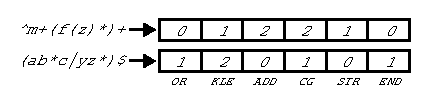
\includegraphics[height=0.6in]{featureUse/illustrations/featureParsing.eps}
\caption{Two patterns parsed into feature vectors}
\label{fig:featureParsing}
\vspace{-12pt}
\end{figure}

Once all patterns were transformed into vectors, we examined each feature independently for all patterns, tracking the number of patterns and  projects that the each feature appears in at least once.




\subsection{Clustering and Behavioral Similarity}
An ideal analysis of regex behavioral similarity would use subsumption or containment analysis. However, we struggled to find a tool that could facilitate such an analysis. Further, regular expressions in code libraries (e.g., for Python, Java) are not the same as regular languages in formal language theory. Some features of regular expression libraries, such as backreferences, make the libraries more expressive than regular languages. This allows a regular expression pattern to match, for example, repeat words, such as ``cabcab", using the pattern {\tt ([a-z]+)\verb!\!1}. However, building an automaton to recognize such a pattern and to facilitate containment analysis, is infeasible.
For these reasons, we developed a similarity analysis based on string matching.


\begin{figure}[tb]
\centering
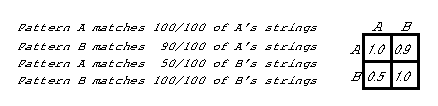
\includegraphics[height=0.6in]{featureUse/illustrations/minimalMatrix.eps}
\caption{A similarity matrix created by counting strings matched}
\label{fig:minimalMatrix}
\end{figure}


\begin{figure}[tb]
\centering
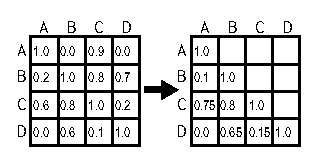
\includegraphics[width=0.7\columnwidth]{featureUse/illustrations/matrixToGraph.eps}
\vspace{-6pt}
\caption{Creating a similarity graph from a similarity matrix}
\vspace{-6pt}
\label{fig:matrixToGraph}
\end{figure}

Our similarity analysis clusters regular expressions by their behavioral similarity on matched strings.
Consider two unspecified patterns {\tt A} and {\tt B}, a set {\tt mA} of 100 strings that pattern {\tt A} matches, and a set {\tt mB} of 100 strings that pattern {\tt B} matches.
If pattern {\tt B} matches 90 of the 100 strings in the set {\tt mA}, then {\tt B} is 90\% similar to {\tt A}.
If pattern {\tt A} only matches 50 of the strings in {\tt mB}, then {\tt A} is 50\% similar to {\tt B}.
We use similarity scores to create a similarity matrix as shown in Figure~\ref{fig:minimalMatrix}.
In row {\tt A}, column {\tt B} we see that {\tt B} is 90\% similar to {\tt A}.
In row {\tt B}, column {\tt A}, we see that {\tt A} is 50\% similar to {\tt B}.  Each pattern is always 100\% similar to itself, by definition.

Once the similarity matrix is built, the values of cells reflected across the diagonal of the matrix are averaged to create a half-matrix of undirected similarity edges, as illustrated in Figure~\ref{fig:matrixToGraph}.
This facilitates clustering using the  Markov Clustering (MCL) algorithm\footnote{\url{http://micans.org/mcl/}}.
We chose MCL  because it offers a fast and tunable way to cluster items by similarity and it is particularly useful when the number of clusters is not known \emph{a priori}.


In the implementation, strings are generated for each pattern using Rex~\cite{rex}.  Rex generates matching strings by representing the regular expression as an automaton, and then passing that automation to a constraint solver that generates members for it\footnote{\url{http://research.microsoft.com/en-us/projects/rex/}}.  If the regex matches a finite set of strings smaller than 400, Rex will produce a list of all possible strings.
Our goal is to generate 400 strings for each pattern to balance the runtime of the similarity analysis with the precision of the similarity calculations.


For clustering, we prune the similarity matrix to retain all similarity values greater than or equal to 0.75, setting the rest to zero, and then using MCL.
This threshold was selected based on recommendations in the MCL manual. The impact of lowering the threshold would likely result  in either the same number of more diverse clusters, or a larger number of clusters, but is unlikely to markedly change the largest clusters or their summaries, which are the focus of our analysis for RQ4 (Section~\ref{rq4:results}), but further study is needed to substantiate this claim.
We also note that MCL can also be tuned using many parameters, including inflation and filtering out all but the top-k edges for each node.
After exploring the quality of the clusters using various tuning parameter combinations, the best clusters (by inspection) were found using an inflation value of 1.8 and k=83.   The top 100 clusters are categorized by inspection into six categories of behavior. % (see Section~\ref{rq4:results}).

The end result is clusters and categories of highly behaviorally similar regular expressions, though we note that this approach has a tendency to over-approximate the similarity of two regexes. We measure similarity based on a finite set of generated strings, but some regexes  match an infinite set (e.g., \verb!ab*c!), so measuring similarity based on the first 400 strings may lead to an artificially high similarity value. To mitigate this threat, we chose a large number of generated strings for each regex, but future work includes exploring other approaches to computing regex similarity.


%\todoNow{fix this before the ICSE deadline - after putting several days into this, I have a partial fix but the fact is there was information loss when going between the java program and the cs program and back again.  So it remains to be seen if it will be feasible to do non-automatic repairs.}
%
%
%We note that there was an operational error in pulling patterns from our database prior to the similarity analysis and clustering, so that 224 patterns (2.3\%) of the 9,727 patterns were omitted. These were duplicate patterns that were quoted differently (for example \verb!`\W'! and \verb!"\W"!).  The result of this error is a slight underestimate in number of projects per pattern (and per cluster), and a slight over-estimate in the pattern, file and project statistics shown in Table~\ref{table:featureStats}.  We do not believe that this error affects our conclusions.



\section{Results}
\label{sec:results}



Next, we present the results of each research question.

\subsection{RQ1: How do developers use regexes?}
\label{rq1:survey}
The survey was completed by 18 participants (82\% response rate) that identified as software developer/maintainers.
Respondents have an average of nine years of programming experience ($\sigma = 4.28$).
On average, survey participants report to compose 172 regexes per year ($\sigma$ = 250) and compose regexes on average once per month, with 28\% composing multiple regexes in a week and an additional 22\% composing regexes once per week. That is, 50\% of respondents uses regexes at least weekly.
Table~\ref{tab:regexenviron} shows how frequently participants compose regexes using each of several languages and technical environments.
Six (33\%) of the survey participants report to compose regexes using general purpose programming languages (e.g., Java, C, C\#) 1-5 times per year and five (28\%) do this 6-10 times per year.  For command line usage in tools such as grep, 6 (33\%) participants use regexes 51+ times per year. Yet, regexes were rarely used in query languages like SQL. Upon further investigation, it turns out the surveyed developers were not on teams that dealt heavily with a database.



%\newcommand{\horiz}{\hspace{2.1pt}}

\begin{table}[t]
\caption{Survey results for number of regexes composed per year by technical environment (RQ1) \label{tab:regexenviron}}
\begin{center}
\begin{small}
\begin{tabular}{l | r @{  \horiz} r @{ \horiz } r @{ \horiz } r @{ \horiz } r @{ \horiz } r }
\toprule
\textbf{Language/Environment} & 0 & 1-5 & 6-10 & 11-20 & 21-50 & 51+ \\  \hline \bigstrut
General  (e.g., Java)  & 1 & 6 & 5 & 3& 1& 2 \\ \hline \bigstrut
Scripting  (e.g., Perl) &5 &4 &3 &3 &2  &1 \\ \hline \bigstrut
Query  (e.g., SQL) & 15&2 &0 &0 &1  & 0\\ \hline \bigstrut
Command line (e.g., grep)   &2 &5 &3 &2 &0  &6 \\ \hline \bigstrut
Text editor (e.g., IntelliJ)   & 2& 5& 0& 5& 1& 5\\
\bottomrule
\end{tabular}
\end{small}
\end{center}
\vspace{-12pt}
\end{table}

\begin{table}
\caption{Survey results for regex usage frequencies for  activities, averaged using a 6-point likert scale: Very Frequently=6, Frequently=5, Occasionally=4, Rarely=3, Very Rarely=2, and Never=1 (RQ1)\label{tab:regexactivities}}
\begin{center}
\begin{small}
\begin{tabular}{l|c}
\toprule
\textbf{Activity} & \textbf{Frequency} \\  \hline \bigstrut
Locating content within a file or files & 4.4\\ \hline \bigstrut
Capturing parts of strings & 4.3 \\ \hline \bigstrut
Parsing user input & 4.0\\ \hline \bigstrut
Counting lines that match a pattern & 3.2\\ \hline \bigstrut
Counting  substrings that match a pattern & 3.2\\  \hline \bigstrut
Parsing generated text & 3.0\\  \hline \bigstrut
Filtering collections (lists, tables, etc.) & 3.0 \\ \hline \bigstrut
Checking for a single character & 1.7\\
\bottomrule
\end{tabular}
\end{small}
\end{center}
\vspace{-12pt}
\end{table}

Table~\ref{tab:regexactivities} shows how frequently, on average, the participants use
regexes for various activities.
Participants answered questions using a 6-point likert scale including very frequently~(6), frequently~(5), occasionally~(4), rarely~(3), very rarely~(2), and never~(1).
%Assigning values from 1 to 6, where 6 is the most frequent, the responses were averaged across participants.
Averaging across participants, among the most common usages are capturing parts of a string and locating content within a file, with both occurring somewhere between occasionally and frequently.

Using a similar 7-point likert scale that includes `always' as a seventh point, developers indicated that they test their regexes with the same frequency as they test their code (average response was 5.2, which is between frequently and very frequently).  Half of the  developers indicate that they use external tools to test their regexes, and the other half indicated that they only use tests that they write themselves. Of the nine developers using tools, six mentioned online composition aides such as \url{regex101.com} where a regex and input string are entered, and the input string is highlighted according to what is matched.
%The other three developers mentioned 'ScalaCheck' (a testing framework), 'IDE regex plugins', and 'Language specific Regexlib'.

When asked an open ended question about pain points encountered with regular expressions, we observed three main categories. The most common, ``hard to compose," was represented in 61\% (11) responses. Next,
 39\% (7) developers responded that regexes are ``hard to read" and 17\% (3) indicated difficulties with ``inconsistency across implementations," which manifest when using regexes in multiple languages. These responses do not sum to 18 as three developers provided multiple parts in their answers.

\vspace{6pt}
\textbf{Summary - RQ1:}
%The survey validates the assumption that regex are widely used by professional software developers and sheds some light into the context in which regexes are used.
%Future research into regex can focus on activities that prove to be most important to developers, namely capturing parts of strings and searching for specific content.
%Although research into regex use in general purpose and scripting languages is important, usage within command line tools and text editors should also be considered.
Common uses of regexes include locating content within a file, capturing parts of strings, and parsing user input.
The fact that all the surveyed developers compose regexes, and half of the developers use tools to test their regexes indicates the importance of tool development for regex.  Developers complain about regexes being hard to read and hard to write.%, and most of the tools that they indicate using are (suitably) focused on composition.

\begin{table}[tb]
\begin{center}
\begin{small}
\caption{How saturated are projects with utilizations? (RQ2)}
\label{table:saturation}

\begin{tabular}{l|ccccc}
\toprule
source & Q1 & Avg & Med & Q3 & Max \\ 
 \hline \bigstrut
utilizations per project & 2 & 32 & 5 & 19 & 1,427 \\ 
 \hline \bigstrut
files per project & 2 & 53 & 6 & 21 & 5,963 \\ 
 \hline \bigstrut
utilizing files per project & 1 & 11 & 2 & 6 & 541 \\ 
 \hline \bigstrut
utilizations per file & 1 & 2 & 1 & 3 & 207 \\ 
\bottomrule
\end{tabular}
\end{small}
\end{center}
\vspace{-12pt}
\end{table}


\subsection{RQ2: How  is the {\tt re} module used?}
We explore regex utilizations and flags used in the scraped Python projects.
Out of the \DTLfetch{data}{key}{nProjScanned}{value}\ projects scanned, \DTLfetch{data}{key}{percentProjectsUsingRegex}{value}\% (\DTLfetch{data}{key}{nProjectsUsingRegex}{value}) contained at least one regex utilization.  To illustrate how saturated projects are with regexes, we measure utilizations per project, files scanned per project, files contained utilizations, and  utilizations  per file, as shown in Table~\ref{table:saturation}.

Of projects containing at least one utilization, the average utilizations per project was 32 and the maximum  was 1,427.  The project with the most utilizations is a C\# project\footnote{\url{https://github.com/Ouroboros/Arianrhod}} that maintains a collection of source code for 20 Python libraries, including larger libraries like {\tt pip}, {\tt celery} and {\tt ipython}.  These larger Python libraries contain many utilizations.
From Table~\ref{table:saturation}, we also see that each project had an average of 11 files containing any utilization, and each of these files had an average of 2 utilizations.



% \begin{figure}[tb]
% \centering
% 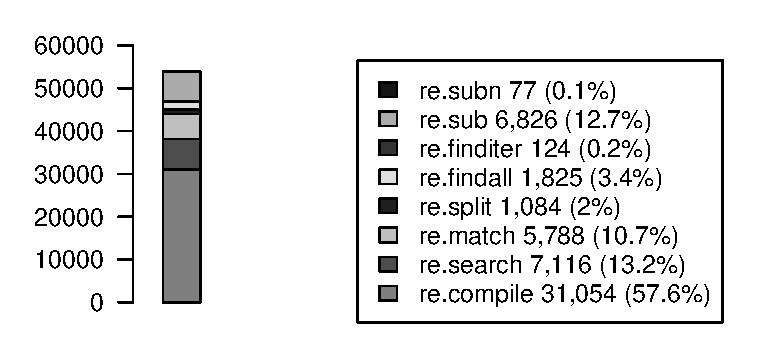
\includegraphics[width=\columnwidth]{featureUse/analysis_output/partFunctions.eps}
% \vspace{-12pt}
% \caption{How often are  {\tt re} functions used? (RQ2)}
% \vspace{-6pt}
% \label{fig:partFunctions}
% \end{figure}

%\begin{figure}[tb]
%\centering
%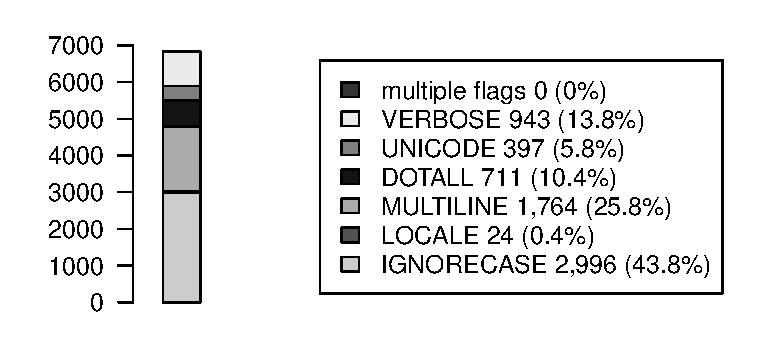
\includegraphics[width=0.9\columnwidth]{../analysis_output/partFlags.eps}
%\vspace{-6pt}
%\caption{Which behavioral flags are used? (RQ2)}
%\vspace{-6pt}
%\label{fig:partFlags}
%\end{figure}

\begin{table*}[h!tb]
\begin{center}
\begin{small}
\caption{How frequently do features appear in projects? (RQ3)}
\label{table:featureStats}
\begin{tabular}{ll@{ }llc @{ } c @{ }c @{ } c  cccccc @{}}
rank & code & description & example & brics & hampi & Rex & RE2 & nPatterns & \% patterns & nProjects & \% projects \\ 
\toprule[0.16em]
1 & ADD & one-or-more repetition & \begin{minipage}{0.5in}\begin{verbatim}z+\end{verbatim}\end{minipage} & \yes & \yes & \yes & \yes & 6,003 & 44.1 & 1,204 & 73.2 \\ 
\midrule
2 & CG & a capture group & \begin{minipage}{0.5in}\begin{verbatim}(caught)\end{verbatim}\end{minipage} & \yes & \yes & \yes & \yes & 7,130 & 52.4 & 1,194 & 72.6 \\ 
\midrule
3 & KLE & zero-or-more repetition & \begin{minipage}{0.5in}\begin{verbatim}.*\end{verbatim}\end{minipage} & \yes & \yes & \yes & \yes & 6,017 & 44.3 & 1,099 & 66.8 \\ 
\midrule
4 & CCC & custom character class & \begin{minipage}{0.5in}\begin{verbatim}[aeiou]\end{verbatim}\end{minipage} & \yes & \yes & \yes & \yes & 4,468 & 32.9 & 1,026 & 62.4 \\ 
\midrule
5 & ANY & any non-newline char & \begin{minipage}{0.5in}\begin{verbatim}.\end{verbatim}\end{minipage} & \yes & \yes & \yes & \yes & 4,657 & 34.3 & 1,005 & 61.1 \\ 
\midrule
6 & RNG & chars within a range & \begin{minipage}{0.5in}\begin{verbatim}[a-z]\end{verbatim}\end{minipage} & \yes & \yes & \yes & \yes & 2,631 & 19.3 & 848 & 51.6 \\ 
\midrule
7 & STR & start-of-line & \begin{minipage}{0.5in}\begin{verbatim}^\end{verbatim}\end{minipage} & \no & \yes & \yes & \yes & 3,563 & 26.2 & 846 & 51.4 \\ 
\midrule
8 & END & end-of-line & \begin{minipage}{0.5in}\begin{verbatim}$\end{verbatim}\end{minipage} & \no & \yes & \yes & \yes & 3,169 & 23.3 & 827 & 50.3 \\ 
\midrule[0.12em]
9 & NCCC & negated CCC & \begin{minipage}{0.5in}\begin{verbatim}[^qwxf]\end{verbatim}\end{minipage} & \yes & \yes & \yes & \yes & 1,935 & 14.2 & 776 & 47.2 \\ 
\midrule
10 & WSP & \textbackslash t \textbackslash n \textbackslash r \textbackslash v \textbackslash f or space & \begin{minipage}{0.5in}\begin{verbatim}\s\end{verbatim}\end{minipage} & \no & \yes & \yes & \yes & 2,846 & 20.9 & 762 & 46.3 \\ 
\midrule
11 & OR & logical or & \begin{minipage}{0.5in}\begin{verbatim}a|b\end{verbatim}\end{minipage} & \yes & \yes & \yes & \yes & 2,102 & 15.5 & 708 & 43 \\ 
\midrule
12 & DEC & any of: 0123456789 & \begin{minipage}{0.5in}\begin{verbatim}\d\end{verbatim}\end{minipage} & \no & \yes & \yes & \yes & 2,297 & 16.9 & 692 & 42.1 \\ 
\midrule
13 & WRD & [a-zA-Z0-9\_] & \begin{minipage}{0.5in}\begin{verbatim}\w\end{verbatim}\end{minipage} & \no & \yes & \yes & \yes & 1,430 & 10.5 & 650 & 39.5 \\ 
\midrule
14 & QST & zero-or-one repetition & \begin{minipage}{0.5in}\begin{verbatim}z?\end{verbatim}\end{minipage} & \yes & \yes & \yes & \yes & 1,871 & 13.8 & 645 & 39.2 \\ 
\midrule
15 & LZY & as few reps as possible & \begin{minipage}{0.5in}\begin{verbatim}z+?\end{verbatim}\end{minipage} & \no & \yes & \no & \yes & 1,300 & 9.6 & 605 & 36.8 \\ 
\midrule
16 & NCG & group without capturing & \begin{minipage}{0.5in}\begin{verbatim}a(?:b)c\end{verbatim}\end{minipage} & \no & \yes & \no & \yes & 791 & 5.8 & 404 & 24.6 \\ 
\midrule
17 & PNG & named capture group & \begin{minipage}{0.5in}\begin{verbatim}(?P<name>x)\end{verbatim}\end{minipage} & \no & \yes & \no & \yes & 915 & 6.7 & 354 & 21.5 \\ 
\midrule
18 & SNG & exactly n repetition & \begin{minipage}{0.5in}\begin{verbatim}z{8}\end{verbatim}\end{minipage} & \yes & \yes & \yes & \yes & 581 & 4.3 & 340 & 20.7 \\ 
\midrule
19 & NWSP & any non-whitespace & \begin{minipage}{0.5in}\begin{verbatim}\S\end{verbatim}\end{minipage} & \no & \yes & \yes & \yes & 484 & 3.6 & 270 & 16.4 \\ 
\midrule
20 & DBB & $n\le x \le m$ repetition & \begin{minipage}{0.5in}\begin{verbatim}z{3,8}\end{verbatim}\end{minipage} & \yes & \yes & \yes & \yes & 367 & 2.7 & 238 & 14.5 \\ 
\midrule
21 & NLKA & sequence doesn't follow  & \begin{minipage}{0.5in}\begin{verbatim}a(?!yz)\end{verbatim}\end{minipage} & \no & \no & \no & \no & 131 & 1 & 183 & 11.1 \\ 
\midrule
22 & WNW & word/non-word boundary & \begin{minipage}{0.5in}\begin{verbatim}\b\end{verbatim}\end{minipage} & \no & \no & \no & \yes & 248 & 1.8 & 166 & 10.1 \\ 
\midrule
23 & NWRD & non-word chars & \begin{minipage}{0.5in}\begin{verbatim}\W\end{verbatim}\end{minipage} & \no & \yes & \yes & \yes & 94 & 0.7 & 165 & 10 \\ 
\midrule
24 & LWB & at least n repetition & \begin{minipage}{0.5in}\begin{verbatim}z{15,}\end{verbatim}\end{minipage} & \yes & \yes & \yes & \yes & 91 & 0.7 & 158 & 9.6 \\ 
\midrule
25 & LKA & matching sequence follows & \begin{minipage}{0.5in}\begin{verbatim}a(?=bc)\end{verbatim}\end{minipage} & \no & \no & \no & \no & 112 & 0.8 & 158 & 9.6 \\ 
\midrule
26 & OPT & options wrapper & \begin{minipage}{0.5in}\begin{verbatim}(?i)CasE\end{verbatim}\end{minipage} & \no & \yes & \no & \yes & 231 & 1.7 & 154 & 9.4 \\ 
\midrule
27 & NLKB & sequence doesn't precede & \begin{minipage}{0.5in}\begin{verbatim}(?<!x)yz\end{verbatim}\end{minipage} & \no & \no & \no & \no & 94 & 0.7 & 137 & 8.3 \\ 
\midrule[0.12em]
28 & LKB & matching sequence precedes & \begin{minipage}{0.5in}\begin{verbatim}(?<=a)bc\end{verbatim}\end{minipage} & \no & \no & \no & \no & 80 & 0.6 & 120 & 7.3 \\ 
\midrule
29 & ENDZ & absolute end of string & \begin{minipage}{0.5in}\begin{verbatim}\Z\end{verbatim}\end{minipage} & \no & \no & \no & \yes & 89 & 0.7 & 90 & 5.5 \\ 
\midrule
30 & BKR & match the $i^{th}$ CG & \begin{minipage}{0.5in}\begin{verbatim}\1\end{verbatim}\end{minipage} & \no & \no & \no & \no & 60 & 0.4 & 84 & 5.1 \\ 
\midrule
31 & NDEC & any non-decimal & \begin{minipage}{0.5in}\begin{verbatim}\D\end{verbatim}\end{minipage} & \no & \yes & \yes & \yes & 36 & 0.3 & 58 & 3.5 \\ 
\midrule
32 & BKRN & references PNG & \begin{minipage}{0.5in}\begin{verbatim}\g<name>\end{verbatim}\end{minipage} & \no & \yes & \no & \no & 17 & 0.1 & 28 & 1.7 \\ 
\midrule
33 & VWSP & matches U+000B & \begin{minipage}{0.5in}\begin{verbatim}\v\end{verbatim}\end{minipage} & \no & \no & \yes & \yes & 13 & 0.1 & 15 & 0.9 \\ 
\midrule
34 & NWNW & negated WNW & \begin{minipage}{0.5in}\begin{verbatim}\B\end{verbatim}\end{minipage} & \no & \no & \no & \yes & 4 & 0 & 11 & 0.7 \\ 
\bottomrule[0.13em]
\end{tabular}
\end{small}
\end{center}
\vspace{-12pt}
\end{table*}


The number of projects that use each of the {\tt re} functions is shown in Figure~\ref{fig:partFunctions}.  The y-axis denotes the total utilizations, with a maximum of \DTLfetch{data}{key}{nUsages}{value}. The {\tt re.compile} function encompasses \DTLfetch{data}{key}{percentCompile}{value}\% of all utilizations. %, presumably because each usage of the other seven functions can accept a regex object compiled using {\tt re.compile} as an argument.
Note that compiled objects can also be used to call functions of the re module, ie {\tt compiledObject.findall(...)}, but we ignore these utilizations so that our analysis is easier to automate, and because we are primarily interested in extracting the patterns which these 8 functions contain.


%When considering flag use, we excluded the default flag, which is built into the {\tt re} module, and present internally whenever no flag is used.
Of all utilizations, \DTLfetch{data}{key}{percentFlags0}{value}\% had no flag, or explicitly specified the default flag.  The debug flag, which causes the {\tt re} regex engine to display extra information about its parsing, was never observed. This may be because developers use it for debugging and choose not to commit it to their repositories.
% Figure~\ref{fig:partFlags} presents the number of projects in which each flag appears. Ignorecase (\DTLfetch{data}{key}{percentI}{value}\%) and multiline (\DTLfetch{data}{key}{percentM}{value}\%) were the most frequently used.   Although multiple flags can be combined using a bitwise or, this was never observed.

\vspace{6pt}
\textbf{Summary - RQ2:}
Only about half of the Python projects sampled contained any utilizations.  Most utilizations used the {\tt re.compile} function to compile a regex object before actually using the regex to find a match.  Most utilizations did not use a flag to modify matching behavior.




%The most frequently observed patterns were used to match whitespace and digits.

\subsection{RQ3: Regex language feature usage}
\label{results:rq3}

We  count the usages of each feature per project and as compared to all distinct regex patterns in the corpus.



\subsubsection{Feature Usage}
\label{sec:featureUsage}
Table~\ref{table:featureStats} displays feature usage from the corpus and relates it to four major regex related projects. Only features appearing in at least 10 projects are listed.
The first column, \emph{rank}, lists the rank of a feature (relative to other features) in terms of the number of projects in which it appears. The next column, \emph{code}, gives a succinct reference string for the feature, and is followed by a \emph{description} column that provides a brief comment on what the feature does.  The \emph{example} column provides a short example of how the feature can be used.
% For example, the most common feature observed in the corpus is \emph{one-or-more repetition}, which is specified in a pattern by using the {\tt +} character in conjunction with some sub-pattern that should repeat one or more times.  The code for this feature is \emph{ADD}, and the short example provided is \verb!z+!.
The next four columns, (i.e., \emph{brics}, \emph{hampi}, \emph{Rex}, and \emph{RE2}), map to the four major research projects chosen for our investigation (see Section~\ref{regextoolsresults}).  We indicate that a project supports a feature with the `\yes' symbol, and indicate that a project does not support the feature with the `\no' symbol.
The final four columns contain two pairs of usage statistics.  The first pair contains the number and percent of \emph{patterns} that a feature appears in, out of the 13,597 patterns that make up the corpus.  The second pair of columns contain the number and percent of \emph{projects} that a feature appears in out of the 1,645 projects scanned that contain at least one utilization.

One notable omission from Table~\ref{table:featureStats} is the literal feature, which is used  to specify matching any specific character.  An example pattern that contains only one literal token is the pattern \verb!`a'!.  This pattern only matches the lowercase letter `a'.  The literal feature was found in \DTLfetch{data}{key}{P_LITERAL_PRESENT}{value}\% of patterns.
%, and accounted for \DTLfetch{data}{key}{P_LITERAL_TOKENS}{value}\% of all tokens.
We consider the literal feature to be necessary for any regex related tool to support, and so exclude it from Table~\ref{table:featureStats} and the rest of the feature analysis.



The eight most commonly used features, ADD, CG, KLE, CCC, ANY, RNG, STR and END,
appear in over half the projects. %The remaining 26 features appear in less than half of the projects containing utilizations.
CG is more commonly used in patterns than the highest ranked feature (ADD) by a wide margin (over 8\%), even though they appear in similar numbers of projects.

\subsubsection{Feature Support in Regex Tools}
\label{regextoolsresults}
While there are many regex tools available, in this work, we focus on the feature support for  four tools, brics, hampi, Rex and RE2, which offer diversity across developers (i.e., Microsoft, Google, open source, and academia) and applications. Further, as we wanted to perform a feature analysis, these four tools and their features are well-documented, allowing for easy comparison.

% We  mapped the features from the corpus to those features supported by the four regular expression engines described in Section~\ref{sec:related}: brics, hampi, RE2, and Rex.
To create the tool mappings, we consulted documentation for each tool. For brics, we collected the set of supported features using the formal grammar\footnote{\url{http://www.brics.dk/automaton/doc/index.html?dk/brics/automaton/RegExp.html}}.  For hampi, we manually inspected the set of regexes included in the {\tt lib/regex-hampi/sampleRegex} file within the hampi repository\footnote{\url{https://code.google.com/p/hampi/downloads/list}} (this may have been an overestimation, as this included more features than specified by the formal grammar\footnote{\url{http://people.csail.mit.edu/akiezun/hampi/Grammar.html}}).  For RE2, we used the  supported feature documentation\footnote{\url{https://re2.googlecode.com/hg/doc/syntax.html}}.  For Rex, we collected the feature set empirically because we tried to parse all scraped patterns with Rex for the behavioral analysis (Section~\ref{rq4:results}), and Rex provides comprehensive error feedback for unsupported features.

%\todoLast{Were there any features supported by the tools that we did not find in the corpus? Answer: RE2 has a lot of features we didn't study and that weren't found in the corpus in any substantial quantity.  I think this is addressed by the earlier mention: Only features appearing in at least 10 projects are listed.}


Of the four projects selected for this analysis, RE2 supports the most studied features (28 features) followed by hampi (25 features),  Rex (21 features), and brics (12 features).  All projects support the 8 most commonly used features except brics, which does not support STR or END.
%All projects support NCC, OR, and the four less common repetition features: QST, SNG, DBB and LWB.  RE2 is the only project to support the WNW, ENDZ and NWNW features.
No projects support the four look-around features LKA, NLKA, LKB and NLKB.  RE2 and hampi support the LZY, NCG, PNG and OPT features, whereas brics and Rex do not.%, which inspired in part the survey questions about feature usage.


\subsubsection{Survey Results for Feature Usage}
The pattern language for Python, which is used to compose regexes, supports default character classes like the ANY or dot character class: \verb!.! meaning, `any character except newline'. % (a full list of features and examples is in the first four columns of Table~\ref{table:featureStats}).
It also supports three other default character classes: \verb!\d!, \verb!\w!, \verb!\s! (and their negations). All of these default character classes can be simulated using the custom character class (CCC) feature, which can create semantically equivalent regexes.
For example  the decimal character class: \verb!\d! is equivalent to a CCC containing all 10 digits:  \verb!\d! $\equiv$ \verb![0123456789]! $\equiv$ \verb![0-9]!.
%Users have a choice when using regex between writing \verb!\d! and \verb![0-9]! and whereas the first option may be shorter, the second may seem more intuitive and readable.
Other default character classes such as the word character class: \verb!\w! may not be as intuitive to encode in a CCC: \verb![a-zA-Z0-9_]!.

Survey participants were asked if they use only CCC, use CCC more than default, use both equally, use default more than CCC or use only default.  Results for this question are shown in Table~\ref{tab:cccvsdefault}, with 67\% (12) indicating that they use default the most.
%Participants were also asked to explain their preferences.
 Participants who favored CCC indicated that ``it is more explicit," whereas the participants who favored default character classes said,  ``it is less verbose" and ``I like using built-in code."



\begin{table}
\caption{Survey results for preferences between custom character and default character classes (RQ3) \label{tab:cccvsdefault}}
\begin{center}
\begin{small}
\begin{tabular}{l|c}
\toprule
\textbf{Preference} & \textbf{Frequency} \\  \hline \bigstrut
use only CCC & 1\\ \hline \bigstrut
use CCC more than default & 5 \\ \hline \bigstrut
use both equally & 2\\ \hline \bigstrut
use default more than CCC & 10\\ \hline \bigstrut
use only default & 2\\
\bottomrule
\end{tabular}
\end{small}
\end{center}
\vspace{-12pt}
\end{table}

To further explore how participants use various regex features, participants were asked five questions about how frequently they use specific related groups of features,
%\begin{itemize} \itemsep -2pt
%    \item endpoint anchors (STR, END): \verb!^! and \verb!$!
%    \item capture groups(CG): (capture me)
%    \item word boundaries (WNW): \verb!word\b!
%    \item (negative) look-ahead/behinds (LKA, NLKA, LKB, NLKB): \verb!a(?=bc)!, \verb!(?<!x)yz!, \verb!(?<=a)!, \verb!a(?!yz)!
%    \item lazy repetition (LZY): \verb!ab+?!, \verb!xy{2,3}?!
%\end{itemize}
%These features were
chosen based on the tool feature support explored in Section~\ref{regextoolsresults}.
Results are shown in Table~\ref{tab:regexfeaturegroups}, indicating that lazy repetition and look-ahead features are rarely used and capture groups and endpoint anchors are occasionally to frequently used.


\begin{table}
\caption{Survey results for regex usage frequencies, averaged using a 6-point likert scale: Very Frequently=6, Frequently=5, Occasionally=4, Rarely=3, Very Rarely=2, and Never=1 (RQ3) \label{tab:regexfeaturegroups}}
\begin{center}
\begin{small}
\begin{tabular}{llc}
\toprule
\textbf{Group} & \textbf{Code} &  \textbf{Frequency} \\  \hline \bigstrut
endpoint anchors & (STR, END) & 4.4\\ \hline \bigstrut
capture groups & (CG) & 4.2 \\ \hline \bigstrut
word boundaries & (WNW) & 3.5 \\ \hline \bigstrut
lazy repetition & (LZY) &  2.9\\ \hline \bigstrut
\multirow{2}{*}{(neg) look-ahead/behind} &  (LKA, NLKA,  & \multirow{2}{*}{2.5}\\
& LKB, NLKB) & \\
\bottomrule
\end{tabular}
\end{small}
\end{center}
\vspace{-12pt}
\end{table}



\vspace{6pt}
\textbf{Summary - RQ3:}
The eight most common features are found in over 50\% of the projects.
%, with two of those not being supported by brics.
%We identify RE2 as the project supporting the most features.%, and identify groups of features supported or not supported by the four regex projects.
%I was confused by the 'at least occasionally' verbage, at first it looked like 'the least occasionally'
Shown in Table~\ref{table:featureStats}, the STR and END features are present in over half of the scanned projects containing utilizations.  In our survey, over half (56\%) of the respondents answered that they use endpoint anchors frequently or very frequently, and none of them claimed to never use them.
%The brics library does not support this feature, which is a missed opportunity for developers who could otherwise have used brics to model their regexes that use STR and END.

The LZY feature  is present in over 36\% of scanned projects with utilizations, and yet was not supported by two of the four major regex projects we explored, brics and RE2.
In our developer survey, 11\% (2) of participants use this feature frequently and 6 (33\%) use it occasionally, showing a modest impact on potential users.

%\subsubsection{PNG and BKRN vs CG and BKR}
%The PNG group (python-style named capture groups) and BKRN (back-references: named) are intended to operate together to allow users to name the content that is expected to appear in a capture group.  A simple example of how these can be used together with the named capture group matching some vowel is:
%\verb!(?P<vowel>[aeiou]x(?P=vowel))! which will match the strings 'axa' and 'oxo' but not 'txt'.  The same functionality can be obtained with a much shorter expression: \verb!([aeiou])x\1! where the \verb!'\1'! references the CG started by the first left parenthesis found when moving from left to right.
When survey participants were asked if they prefer to always use numbered (BKR) or named (BKRN) back references, 66\% (12) of survey participants said that they always use BKR, and the remaining 33\% (6) said ``it depends."  No participants preferred named capture groups.  BKR is present in 5\% of scanned projects, while BKRN is present in only 1.7\%, which corroborates our findings that numbered  are generally preferred over named capture groups.

\subsection{RQ4: Regex behavioral similarity}
\label{rq4:results}


In clustering the regular expressions, we are most interested in observing behavior of regexes found in multiple projects.  Starting with the 13,597 patterns of the corpus, we discarded 10,015 (74\%) patterns that were not found in multiple projects.
Then we excluded an additional 711 (5\%) patterns that contain features not supported by Rex.  We studied the remaining 2,871 (21\%) patterns using our similarity analysis technique. The impact is that 923 projects were excluded from the data set for the similarity analysis. Omitted features are indicated in Table~\ref{table:featureStats} for Rex.
%The generated strings for each pattern are used to measure the pairwise similarity for all patterns and construct the similarity matrix.


%\subsubsection{Rationale for Behavioral Clustering}


%\subsubsection{General Information About Clusters Found}
From 2,871 distinct patterns, MCL clustering identified 186 clusters with 2 or more patterns, and 2,042 clusters of size 1.
%Recall that only pairs of patterns with a similarity level of 0.75 were included in the matrix passed to MCL.
 The average size of clusters larger than size one was 4.5.  Each pattern belongs to exactly one cluster.

%\subsubsection{An Example Cluster}

%Three example strings generated by Rex for the first pattern are: `-()', `*'8(5)', `Oe()'.  For the third pattern, Rex generated these three strings: ` ()', `(q)F', `(n)M'.  The pattern: \verb!\(.*\)$! is very similar, but will not match the string `(n)M', and so was placed in a different cluster.

\begin{table}
\begin{center}
\caption{Sample from an example cluster (RQ4)}
\label{table:exampleCluster}
\begin{small}
\begin{tabular}
{lcc | lcc}
\toprule
index & pattern & nProjects & index & pattern & nProjects \\
 \hline \bigstrut
1 & \begin{minipage}{0.3in}\begin{verbatim}`:+'\end{verbatim}\end{minipage} & 8 & 5 & \begin{minipage}{0.5in}\begin{verbatim}`[:]'\end{verbatim}\end{minipage} & 6 \\
 \hline \bigstrut
2 & \begin{minipage}{0.3in}\begin{verbatim}`(:)'\end{verbatim}\end{minipage} & 8 & 6 & \begin{minipage}{0.6in}\begin{verbatim}`([^:]+):(.*)'\end{verbatim}\end{minipage} & 6 \\
 \hline \bigstrut
3 & \begin{minipage}{0.3in}\begin{verbatim}`(:+)'\end{verbatim}\end{minipage} & 8 & 7 & \begin{minipage}{0.5in}\begin{verbatim}`\s*:\s*'\end{verbatim}\end{minipage} & 4 \\
 \hline \bigstrut
4 & \begin{minipage}{0.3in}\begin{verbatim}`(:)(:*)'\end{verbatim}\end{minipage} & 8 & 8 & \begin{minipage}{0.5in}\begin{verbatim}`\:'\end{verbatim}\end{minipage} & 2 \\
\bottomrule
\end{tabular}
\vspace{-6pt}
\end{small}
\end{center}
\vspace{-12pt}
\end{table}


%
%\begin{table}
%\begin{center}
%\caption{An example cluster (RQ3)}
%\label{table:exampleCluster}
%\begin{small}
%\begin{tabular}
%{lcc}
%\toprule
%index & pattern & nProjects\\
%\midrule
%1 & \begin{minipage}{0.5in}\begin{verbatim}`\s*,\s*'\end{verbatim}\end{minipage} & 54  \\
%\midrule
%2 & \begin{minipage}{0.5in}\begin{verbatim}`,'\end{verbatim}\end{minipage} & 30 \\
%\midrule
%3 & \begin{minipage}{0.5in}\begin{verbatim}`\s*,'\end{verbatim}\end{minipage} & 16 \\
%\midrule
%4 & \begin{minipage}{0.5in}\begin{verbatim}` ,\s*'\end{verbatim}\end{minipage} & 13 \\
%\midrule
%5 & \begin{minipage}{0.5in}\begin{verbatim}` *, *'\end{verbatim}\end{minipage} & 12 \\
%\midrule
%6 & \begin{minipage}{0.5in}\begin{verbatim}`,\S'\end{verbatim}\end{minipage} & 5 \\
%\midrule
%7 & \begin{minipage}{0.5in}\begin{verbatim}`,.*$'\end{verbatim}\end{minipage} & 3 \\
%\midrule
%8 & \begin{minipage}{0.6in}\begin{verbatim}`(\S+)\s*,\s*'\end{verbatim}\end{minipage} & 2 \\
%\midrule
%9 & \begin{minipage}{0.5in}\begin{verbatim}`,+'\end{verbatim}\end{minipage} & 1 \\
%\midrule
%10 & \begin{minipage}{0.5in}\begin{verbatim}`,\ ?'\end{verbatim}\end{minipage} & 1 \\
%\midrule
%10 & \begin{minipage}{0.5in}\begin{verbatim}`,\s*(\S)'\end{verbatim}\end{minipage} & 1 \\
%\midrule
%11 & \begin{minipage}{0.5in}\begin{verbatim}`\s*(,)\s*'\end{verbatim}\end{minipage} & 1 \\
%\midrule
%12 & \begin{minipage}{0.5in}\begin{verbatim}`\s*\,\s*'\end{verbatim}\end{minipage} & 1 \\
%\bottomrule
%\end{tabular}
%\end{small}
%\end{center}
%\end{table}


%\subsubsection{Using the Smallest Pattern to Represent a Cluster}

Table~\ref{table:exampleCluster} provides an example of a behavioral cluster containing 12 patterns (four longer patterns omitted for brevity). Patterns from this cluster are present in 31 different projects.  All patterns in this cluster share the literal `:' character. The smallest pattern, \verb!`:+'!,  matches one or more colons.


% \begin{figure}[tb]
% \centering
% 
\includegraphics[width=\columnwidth]{../illustrations/clusterEdgesExample.eps}
% \vspace{-12pt}
% \caption{Example Of Similarity Edges Of One Cluster}
% \vspace{-6pt}
% \label{fig:clusterEdgesExample}
% \end{figure}


%Another pattern from this cluster, \verb!([^:]+):(.*)!, requires at least one non-colon character to occur before a colon character.  Our similarity value between these two regexes was below the minimum of 0.75 because Rex generated many strings for `:+' that start with one or more colons.
% Todo: create a graph graphic with edge weights showing similarity values for all 8 of these patterns.
We observe that the smallest pattern in a cluster provides insight about key characteristic that all the patterns in the cluster have in common.  A shorter pattern will tend to have less extraneous behavior because it is specifying less behavior,
yet, in order for the smallest pattern to be clustered, it had to match most of the strings created by Rex from many other patterns within the cluster, and so we observe that {the smallest pattern is useful as a representative of the cluster}.

For the rest of this paper, a cluster will be represented by one of the shortest patterns it contains, followed by the number of projects any member of the cluster appears in, so the cluster in Table~\ref{table:exampleCluster} will be represented as \verb!`:+'(31)!.  This representation is not an attempt to express all notable behavior of patterns within a cluster, but is a useful and meaningful abbreviation.
Other regexes in the cluster may exhibit more diverse behavior, for example the pattern \verb!`([^: ]+):(.*)'! requires a non-colon character to appear before a colon character.

We manually mapped the top 100 largest clusters based on the number of projects into 6 behavioral categories (determined by inspection).  The largest cluster was left out, as it was composed of patterns that trivially matched almost any string, like \verb!`b*'! and \verb!`^'!.  The remaining 99 clusters were all categorized. These clusters are briefly summarized in Table~\ref{tab:clustercats}, showing the name of the category and the number of clusters it represents, patterns in those clusters, and projects. The most common category is \emph{Multi Matches}, which contains clusters that have alternate behaviors (e.g., matching a comma or a semicolon, as in \verb!`,|;'(18)!). Each cluster was mapped to exactly one category. Next, we describe the categories, ordered by the number of projects the regex patterns map to.

%When a cluster can fit in multiple categories, it is placed in the most specific category.  The following six categories are listed in order from most specific behavior to least specific behavior.

\begin{table}
\begin{center}
\begin{small}

\caption{Cluster categories and sizes (RQ4) \label{tab:clustercats}}
\begin{tabular}{lccc}
\toprule
\textbf{Category} & \textbf{Clusters} & \textbf{Patterns} & \textbf{Projects} \\  \hline \bigstrut
Multi Matches & 21 & 237 & 295\\
\hline \bigstrut
Specific Char & 17 & 103 & 184\\
\hline \bigstrut
Anchored Patterns & 20 & 85 & 141\\
\hline \bigstrut
 Content of Parens & 10 & 46 & 111\\
\hline \bigstrut
Two or More Chars & 16 & 40 & 120\\
\hline \bigstrut
Code Search & 15 & 27 & 92 \\
\bottomrule
\end{tabular}
\vspace{-12pt}
\end{small}
\end{center}
\end{table}

%6
\subsubsection{Multiple Matching Alternatives}
The patterns in these clusters match under a variety of conditions by using a character class or a disjunctive \verb!|!.
For example:
\verb!`(\W)'(89)! matches any alphanumeric character, \verb!`(\s)'(89)! matches any whitespace character, \verb!`\d'(58)! matches any numeric character, and \verb!`,|;'(18)! matches a comma or semicolon.  Most of these clusters are represented by patterns that use default character classes, as opposed to custom character classes.  This provides further support for our survey results to the question, \emph{Do you prefer to use custom character classes or default character classes more often?}, in which a majority of participants indicated they use the default classes more than custom.
%This category contains 21 clusters, each appearing in an average of 33 projects.
%Todo: this category is the most general, and has 2 sub-catagories of small CCCs and very large ranges/complex CCCs.
%These clusters have a combined total of 237 patterns, with at least one pattern present in 295 projects.


%5
\subsubsection{Specific Character Must Match}
\label{cluster:single}
Each cluster in this category requires one specific character to match, for example:
\verb!`\n\s*'(42)! matches only if a newline is found, \verb!`:+'(31)! matches only if a colon is found, \verb!`%'(22)!, matches only if a percent sign is found and \verb!`}'(14)! matches only if a right curly brace is found.
Table~\ref{table:exampleCluster} presents a cluster that falls under this category.
% \todoMid{Repair after merge conflict later}
% Table~\ref{table:exampleCluster} presents a cluster that falls under this category. While the cluster is centered on the presence of the \verb!`:'! character, the other regexes in the cluster also exhibit more diverse behavior.
The commonality of this cluster category contrasts with the survey in Section~\ref{rq1:survey} in which participants reported to very rarely or never use regexes to check for a single character (Table~\ref{tab:regexactivities}).
%This category contains 17 clusters, each appearing in an average of 17.1 projects.
% These clusters have a combined total of 103 patterns, with at least one pattern present in 184 projects.

%3
\subsubsection{Anchored Patterns}
Each of the clusters uses at least one endpoint anchor to require matches to be absolutely positioned, for example:
\verb!`(\w+)$'(35)! captures the word characters at the end of the input, \verb!`^\s'(16)! matches a whitespace at the beginning of the input, and \verb!`^-?\d+$'(17)! requires that the entire input is an (optionally negative) integer.
These anchors are the only way in regexes to guarantee that a character does (or does not) appear at a particular location by specifying what is allowed. As an example, \verb!^[-_A-Za-z0-9]+$! says that from beginning to end, only \verb![-_A-Za-z0-9]! characters are allowed, so it will fail to match if undesirable characters, such as \verb!?!, appear anywhere in the string.
%This category contains 20 clusters, each appearing in an average of 15.4 projects.
%These clusters have a combined total of 85 patterns, with at least one pattern present in 141 projects.

%\todoMid{The thing I want to mention about anchored patterns (but have struggled to say in the past) is that they are the only way to guarantee that a character does not appear in a particular location by specifying what is allowed.  Consider the regex }
%\verb!^[-_A-Za-z0-9]+$!
%\todoMid{ which will fail to match if an undesirable character like `?' appears anywhere in the input.  In logic, there is a similar phenomenon.  That is, `Always' is true iff `Not Exists' of the negation is true, and by requiring an entire input to always maintain some abstraction, you can indirectly specify the negation of another (inverse) abstraction.  Even with only one anchor point, a regex like }
%\verb!.*[0-9]$!
%\todoMid{ is creating an ultimatum about the end being a digit.  Without the endpoint anchors, I don't see how one could specify absolutes about an input. }

%2
\subsubsection{Content of Brackets and Parenthesis}
\label{cluster:contentparens}
The clusters in this category center around finding a pair of characters that surround content, often also capturing that content. For example,
\verb!`\(.*\)'(29)! matches when content is surrounded by parentheses and \verb!`".*"'(25)! matches  when content is surrounded by double quotes.  The cluster \verb!`<(.+)>'(23)! matches and captures content surrounded by angled brackets.
%This category contains 10 clusters, each appearing in an average of 18.4 projects.
% These clusters have a combined total of 46 patterns, with at least one pattern present in 111 projects.
%, and \verb!`\[.*\]'(22)! matches when content is surrounded by square brackets
%4
\subsubsection{Two or More Characters in Sequence}
\label{cluster:multiple}
These clusters require several characters in a row to match some pattern, for example:
\verb!`\d+\.\d+'(30)! requires one or more digits followed by a period character, followed by one or more digits.  The cluster \verb!`  '(17)! requires two spaces in a row,
%\verb!`([A-Z][a-z]+[A-Z][^ ]+)'(11)!,
and \verb!`@[a-z]+'(9)! requires the at symbol followed by two or more lowercase characters, as in a twitter handle.
%This category contains 16 clusters, each appearing in an average of 13 projects.
%These clusters have a combined total of 40 patterns, with at least one pattern present in 120 projects.

%\todoMid{Again, it might be interesting to look at what particular sequences are looking like.  I think I mention this again in the discussion, but should we put it here instead?}

%1
\subsubsection{Code Search and Variable Capturing}
\label{cluster:search}
These clusters show a recognizable effort to parse source code or URLs. For example,
\verb!`^https?://'(23)! matches a web address, and \verb!`(.+)=(.+)'(9)! matches an assignment statement, capturing both the variable name and value.
The cluster  \verb!`\$\{([\w\-]+)\}'(11)! matches an evaluated string interpolation and captures the code to evaluate.
%This category contains 15 clusters.%, each appearing in an average of 11.7 projects.
%These clusters have a combined total of 27 patterns, with at least one pattern present in 92 projects.

\vspace{6pt}
\textbf{Summary - RQ4:}
%When tool designers are considering what features to include, data about usage in practice is valuable.  Behavioral similarity clustering  helps to discern these behaviors by looking beyond the structural details of specific patterns and seeing trends in  matching behavior. % We are also able to find out what features are being used in these behavioral trends so that we can make assertions about why certain features are important.
%We used the behavior of individual patterns to form clusters, and identified six main categories for the clusters.
% Overall, we see that many clusters are defined by the presence of particular tokens, such as the colon for the cluster in Table~\ref{table:exampleCluster}.
We identified six main categories that define regex behavior at a high level: matching with alternatives, matching literal characters, matching with sequences, matching with endpoint anchors, parsing contents of brackets or braces, or searching and capturing code. %, and can be considered in conjunction with the self-described regex activities from the survey in Table~\ref{tab:regexactivities} to be representative of common uses for regexes.
%One of the six common cluster categories, \emph{Code Search and Variable Capturing}, has a very specific purpose of parsing source code files. This shows a very specific and common use of regular expressions in practice.




\section{Discussion}
\label{sec:discussion}

In this section, we discuss the implications of these empirical findings
%on tool designers and users of regex tools
 and opportunities for future work.

\subsection{Implications For Tool Designers}
The results have  implications for regex tool designers. % who want to effectively support developers who use regular expressions.

%\subsubsection{All Character Classes Are Common}
%The same character class can be expressed in different ways, for example \verb!`[0-9]'! is equivalent to \verb!`\d'!.  Our results indicate that both approaches are widely used (Table~\ref{tab:cccvsdefault}), so tool builders should continue to support both approaches.


\subsubsection{Finding Specific Content}
Two categorical clusters, \emph{Specific Characters Must Match} (Section~\ref{cluster:single}) and \emph{Two or More Characters in Sequence} (Section~\ref{cluster:multiple}), deal with identifying the presence of specific character(s).
While multiple character matching subsumes single character matching, the overarching theme is that these regexes are looking to validate strings based on the presence of very specific content, as would be done for many common activities listed in Table~\ref{tab:regexactivities}, such as, ``Locating content within a file or files."
%(This is in contract to \emph{capturing} specific content, as \emph{finding} deals with string validation and \emph{capturing} deals with string extraction.)
%As indicated by the clusters of specific character matches in Section~\ref{cluster:single}, finding specific content is important.
%Delimiters that separate items on one line like \verb!`\t'! are also quite common.
%Although survey participants indicated an average frequency of 1.7 (very rarely or never) for ``checking for a single character," we found that 17 of the top 100 clusters revolved around the presence of a single character.
%The commonality of regexes related to finding content is consistent with the top ranked activity for developers, ``Locating content within a file or files."
%and usually this content is located using some small set of characters that the user knows will flag that content.
More study is needed into what content is most frequently searched for, but from our cluster analysis we found that version numbers, twitter or user handles, hex values, decimal numbers, capitalized words, and particular combinations of whitespace, slashes and other delimiters were discernible targets.

%Looking closely at the \emph{Specific Character Must Match} cluster, some of the characters being searched for were \verb!\n!, \verb!-! and \verb!.!, which are all common delimiters in different scenarios. This indicates the need for regex tools to facilitate easy file parsing, or for tools to include built-in support for specific, common types of parsing.


\subsubsection{Capturing Specific Content Near A Delimiter}
The survey results from Section~\ref{rq1:survey} indicate that capturing parts of strings is among the most frequent activities for which developers use regexes.
From a feature perspective, the capture group (CG) is the most frequently used in terms of patterns (Table~\ref{table:featureStats}).  This feature has two functions: 1) logical grouping as would be expected by parenthesis, and 2) retrieval of information in one logical grouping.  As mentioned in Section~\ref{rq4:results}, capturing content was a primary goal evident in several cluster categories.  The fourth-largest category is based entirely on capturing the content between brackets or parentheses (Section~\ref{cluster:contentparens}).

%Combined with the cluster on \emph{Code Search and Variable Capturing} (Section~\ref{cluster:search}), this emphasizes the need for regex tools to  facilitate easy file parsing, or for a tool to include built-in support for specific, common types of parsing.


Many uses of CG also use the ANY and KLE features, eg. \verb!(.*){(.*)}(.*)! and \verb!\\s*([^: ]*)\\s*:(.*)!.  This type of usage frequently revolves around an important delimiter character such as \verb!:! or \verb!\!.  This use case is well supported by existing tools for ASCII characters, but future tools should consider the centrality of this use case and its implications for non-English users of regex tools.  For example, Unicode characters like `U+060D' the Arabic Date Separator, or `U+1806' the Mongolian Todo Soft Hyphen may be used to locate segments of text that a user would want to capture.

%, such as finding a twitter handle (i.e., \verb!@[a-z]+!) or a version number, (i.e., \verb!v[0-9]+.*!).
%and then capture specific content, such as the actual twitter handle or the actual version number, but may not know how to do that capture groups and may rely on string parsing instead.

%\todoMid{The main difference between the Specific Character Must Match group and the multiple characters must match is that the first can subsume the second.  I think it's important to defend this and expose that we understand that our simplification of clusters to their shortest representative combined with the behavioral clustering technique will drastically over-emphasize similarities revolving around single characters, so instead of listing this as a major group, or a major finding, we may need to admit that it is an emphasis that our technique introduces artificially.  I think that in practice, the patterns being searched for usually revolve around more than just a single character, although maybe not a lot more than that.  I think it is more telling that despite our technique's tendency to over-cluster things around a single character, there was still an entire category that required two or more characters, and so those specific pairs or triples or whatever in that cluster are extremely key character combinations.  Let's see a few of those that seem to make sense: }
%\verb! {2,}!
%\todoMid{ :two or more spaces, }
%\verb!@[a-z]+!
%\todoMid{ :a lowercase twitter handle or similar,}
% \verb!\\$[()]!
% \todoMid{ :a dollar followed by either paren, }
% \verb!v[0-9]+.*!
% \todoMid{ :the letter `v' followed by some numbers, perhaps a version number.  }

\subsubsection{Counting Lines}
Text files containing one unit of information per line are common in a wide variety of applications (for example .log and .csv files).  Out of the 13,597 patterns in the corpus, 3,410 (25\%) contained ANY followed by KLE  (i.e., \verb!`.*'!), often at the end of the pattern.
One reasonable explanation for this tendency to put \verb!`.*'! at the end of a pattern is that users want to disregard all matches after the first match on a single line in order to count how many distinct lines the match occurs on.  Survey participants indicated an average frequency of ``Counting lines that match a pattern" and ``Counting substrings that match a pattern" at 3.2 or rarely/occasionally. It may be valuable for tool builders to include support for common activities such as line counting.



%\todoMid{In a completely unrelated train of thought, I have been considering how regexes are one major way, and perhaps the only practical way in the world of computer science to handle the invisible characters like ASCII 0-32.  That's 33 characters like `backspace' and `end of medium' and 'vertical tab' that can appear in text and cause problems.  I've heard them called `Gremlins'.  So what do people do?  They write regexes to clean those out.}



\subsection{Opportunities For Future Work}

There are many opportunities for future work. %\todoLast{Hey Kids! Need a thesis topic? Here's a bunch! Promote this awesome section earlier}




\subsubsection{Refactoring Regexes}
The survey showed that users want readability and find the lack of readable regexes to be a major pain point.
This provides an opportunity to introduce refactoring transformations to enhance readability or comprehension.
As one opportunity, certain character classes are logically equivalent and can be expressed differently, for example, \verb!\d! $\equiv$ \verb![0123456789]! $\equiv$ \verb![0-9]!. While \verb!\d! is more succinct, \verb![0-9]! may be easier to read, so a refactoring for \emph{default to custom character classes} could be introduced.
Human studies are needed to evaluate the readability and comprehension of various regex features in order to define and support appropriate regex refactorings.

Another avenue of refactoring could be for performance. Various implementations of regex libraries may perform more efficiently with some features than others. An evaluation of regex feature implementation speeds would facilitate semantic transformations based on performance, similar to performance refactorings for LabVIEW~\cite{chambers2013smell, chambers2015impact}.


Additionally, some developers may  \emph{find} specific content with a regex  and then subsequently \emph{capture} it with string parsing, which may be more error prone than using a capture group and indicates a missed opportunity to use the full extent of regex libraries. Future work will explore source code to identify the frequency of such occurrences and design refactorings to better utilize regex library features.

%Other similar refactoring techniques may become evident with a more thorough search.  A tool that preserved the exact behavior of a regex but optimized for readability could be incorporated into an IDE and relieve some developer pain.  More research is needed into why certain character classes are considered more readable, as has been done for other refactoring work (e.g.,~\cite{StoleeTSE2013}).
%Similarly, there are several principals that can be followed to enhance the performance of a regex.  Using non-capture groups whenever possible, avoiding backtracking, etc.  In theory it seems possible to build a compiler that could compose a regex with identical behavior but with better readability and performance.

\vspace{-2pt}
\subsubsection{Migration  Support for Developers}
Within standard programming languages, regular expressions libraries are very common, yet there are subtle  differences between language libraries in the supported features. For example, Java supports possessive quantifiers like \verb! `ab*+c'! (here the `+' is modifying the `*' to make it possessive) whereas Python does not. Differences among programming language implementations was identified as a pain point for using regular expressions by 17\% of the survey participants. This provides a future opportunity for tools that translate between regex utilizations in various languages.

\vspace{-2pt}
\subsubsection{Similarity Beyond String Matching}
There are various ways to compute similarity between regexes, each with different tradeoffs.
While the similarity analysis we employ over-approximates similarity when compared to containment analysis, it may under-approximate similarity in another sense.
%We define behavioral similarity based on strings matched by pairs of regular expressions. However, t
For example, two regexes that have dissimilar matching behavior could be very similar in purpose and in the eyes of the developer. For example, \verb!commit:\[(\d+)\] - (.*)! and \verb!push:\[(\d+)\] - (.*)! could both be used to  capture the id and command from a versioning system, but match very different sets of strings. Future work would apply abstractions to the regex strings, such as removing or relaxing literals, prior to similarity analysis to capture and cluster such similarities.

From another perspective, our regex similarity measure, and even containment analysis, could treat behaviorally identical regexes as the same, when  their usage in practice is completely different. For example, in Table~\ref{table:exampleCluster}, the regexes \verb!`:+'! and \verb!`(:+)'! are behaviorally identical in that they match the same strings, except the latter uses a capture group. In practice, these may be used very differently, where the former may be used for validation and the latter for extraction. This usage difference could be observed by code  analysis, and is left for future work.

\vspace{-2pt}
\subsubsection{Automated Regex Repair}
Regular expression errors are common and have produced thousands of bug reports~\cite{Spishak:2012:TSR:2318202.2318207}. This provides an opportunity to introduce automated repair techniques for regular expressions.
Recent approaches to automated program repair rely on mutation operators to make small changes to source code and then re-run the test suite (e.g., ~\cite{cacm10, genprog-tse-journal}). In regular expressions, it is likely that the broken regex is close, semantically, to the desired regex. Syntax changes through mutation operators could lead to big changes in behavior, so we hypothesize that using the semantic clusters identified in Section~\ref{rq4:results} to identify potential repair candidates could efficiently and effectively converge on a repair candidate.

\subsubsection{Developer Awareness of Best Practices}
One category of clusters, \emph{Content of Brackets and Parenthesis}, parses the contents of angle brackets, which may indicate developers are using regexes to parse HTML or XML.  As the contents of angle brackets are usually unconstrained, regexes are a poor replacement for XML or HTML parsers.  This may be a missed opportunity for the regex users to take advantage of more robust tools. More research is needed into how regex users discover best practices and how aware they are of how regexes should and should not be used.
%http://english.stackexchange.com/questions/50851/the-contents-are-or-the-contents-is

%\subsubsection{Support for Regexes Composition}
%According to our survey, over 60\% of developers find regexes to be difficult to compose. Additionally, developers frequently or very frequently write tests for their regexes. This provides an opportunity to instead





\subsubsection{Tool-Specific Regex Exploration}
In some environments, such as command line or text editor, regexes are used extensively by the surveyed developers (Section~\ref{rq1:survey}), but these regular expressions do not persist. Thus, using a repository analysis for feature usage only illustrates part of how regexes are used in practice. Exploring how the feature usage differs between environments would help inform tool developers about how to best support regex usage in context, and is left for future work.


% \subsubsection{A Modern WRD Character Class}
% \todoMid{update}
% One unexpected result of our clustering is that, behaviorally speaking, the negation of the word class NWRD was used in 208 projects, while the word class itself was used in only 114 projects. After inspecting several projects using the patterns found in this behavioral cluster, we concluded that most users are trying to sanitize arbitrary strings that must conform to a system character set requirement, such as requirements for filenames.  For example, a user might replace all NWRD matching characters with the `\_' to guarantee that an arbitrary string can be used as a filename.  We also considered the largest cluster using custom character classes (\verb?`[^ -~]'(122)?) and concluded that users are constructing a more permissive version of the NWRD character class, to allow more non-letter, non-digit characters than just the `\_' in their sanitized strings.  More research is needed to determine if a more modern WRD class could be useful, and if so, what characters set is preferred.




\section{Threats to Validity}
\label{sec:threats}
The following threats impact our results and conclusions:

%\subsection{Conclusion}
\textbf{Reliability of Measures:} The validity of our survey results is dependent on the clarity of the questions. The authors went through several iterations of the survey and included examples for all the regex feature descriptions to improve understandability.

The similarity measure between regexes used in the cluster algorithm is computed empirically rather than analytically, and the more Rex-generated strings used to compute the similarity measure, the more likely it is to be accurate. Our experiments used 400 strings to balance performance and precision, but a higher number could lead to more cohesive clusters. Additionally, regex patters that use any feature not supported by Rex were omitted from the cluster analysis. Last, the threshold of 0.75 was chosen based on the MCL recommendation, but it may not create optimal clusters. %\todoMid{talk about tools for formal analysis}
%In our clustering algorithm, we require a similarity level of 0.75 so that we do not over-estimate the similarity between regular  expressions.\todoNow{what does this last sentence mean?  Is this paragraph okay?}

%\subsection{Internal}

\textbf{Instrumentation:} Regular expression patterns were clustered using strings generated by the Rex tool.  We assume that the strings generated by Rex are reasonably diverse to help characterize the regex behavior. To mitigate this threat, Rex generated 400 strings per regex and we inspected strings randomly to ensure diversity.

Implementation errors are a risk for research involving repository analysis. To combat this, we have tested our code and made the repository publicly available\footnote{GitHub link removed for anonymity}.%\url{https://github.com/softwarekitty/tour_de_source}}.

\textbf{Selection:} We mined \DTLfetch{data}{key}{nProjScanned}{value} Python projects from GitHub, which is  small compared to all available projects with Python code. The projects were mined using the GitHub API which sorts the projects by creation date. By using the API, the goal was to reduce  sampling bias from the researchers.

We also did not scrape all commits in every project for regular expression utilizations, rather, we grabbed each project every 20 commits. It is possible that in between the scanned commits, a regex utilization was added and then removed, leading to fewer utilizations in our final data set.

\textbf{Recall bias:} Survey participants were asked to reflect on their past behavior, which may not  represent actual behavior. To mitigate this, we designed the survey to lead participants to think about their behavior before summarizing (e.g., asking how often they use regexes in each of several environments before asking about usage frequency).

%\subsection{Construct}

%\textbf{Hypothesis guessing:} The lead author was an employee of Dwolla when the survey was run, so participant behavior may have been affected by their relationship with the author. To combat this, the beginning of the survey stated, ``As this is for research, please answer as accurately as possible, not guessing what is the desired answer and providing that."

%\subsection{External}

\textbf{Interaction of Selection and Treatment:} Our survey participants were software developers from a small startup company and may not be representative of developers who use regexes. Given that the average participant has nine years of development experience, their responses likely pull from a variety of experiences with regular expression usage, but replication with a more diverse set of developers is needed.

\textbf{Interaction of Setting and Treatment:}
We only explore regular expressions in Python projects so these results may be coupled with the activities performed using Python and not generalize to other languages. The regex usage context reported by survey participants, however, includes information on  regex usage in a  variety of settings and languages. Future work will replicate this study in other languages.



%The survey results are from a set of developers at one company and may not generalize to other developers at that company or at other companies. While the results provide some information on regex usage, repeating the survey to a larger set of diverse developers will increase the generalizeability of the results.
%%
%
%In extracting patterns for analysis, we omit utilizations that contain flags since flags provide refinements on the functionality of the pattern as it is used in the project. Given that only 12.7\% of all utilizations used flags, the impact on the clusters should be minimal.
%
%%The feature analysis is dependent on the features identified in the PCRE parser.
%


%\vspace{-6pt}
\section{Conclusion}
\label{sec:conclusion}
In this work, we have explored the contexts in which regular expressions are used as well as the features and behavioral similarities of regexes found in open source Python projects. In a survey of 18 professional developers, we find that 50\% compose regular expressions at least weekly. The most common purposes are locating content within a file or capturing parts of strings. The most difficult parts about working with regular expressions were reported to be composing and reading them.
In a study of regular expression usage in nearly 4,000 Python projects, we find that over 42\% of projects contain a regular expression.
We present an approach to measure behavioral similarity between regexes by generating strings that match one regex and pairwise  testing the remaining regexes against it. This similarity measure is used to form cross-project behavioral clusters. In the top 100 largest clusters, we find that capturing the contents of brackets,  searching for delimiter characters and matching alternative values were common behaviors.
These results have implications for tool designers and for future research aimed at better supporting developers in using regular expressions.


% use section* for acknowledgement
%\vspace{-6pt}
\section*{Acknowledgment}
%\vspace{-2pt}
Special thanks to the Dwolla developers for their survey participation.
This work is supported in part by NSF SHF-1218265, NSF SHF-EAGER-1446932, and the Harpole-Pentair endowment at Iowa State University.

%\vspace{12pt}
\newpage
\bibliographystyle{abbrv}

% The bibliography should be embedded for final submission.
\balance
\bibliography{biblio}



% that's all folks
%\end{document}


\chapter{Refactoring}
%\documentclass{sig-alternate-05-2015}

%\begin{document}
%\bstctlcite{IEEEexample:BSTcontrol}
%
% paper title
% can use linebreaks \\ within to get better formatting as desired
% \title{Refactoring Regular Expressions}


% \numberofauthors{2}
% \author{
% % 1st. author
% \alignauthor
% Carl Chapman\\
%        \affaddr{Department of Computer Science}\\
%        \affaddr{Iowa State University}\\
%        \email{carl1976@iastate.edu}
% \alignauthor
% Kathryn T. Stolee\\
%        \affaddr{Department of Computer Science}\\
%        \affaddr{North Carolina State University}\\
%        \email{ktstolee@ncsu.edu}
% \alignauthor
% }


% \maketitle


\begin{abstract}
Regular expressions (regex) are powerful tools employed across many tasks and platforms.
Regex can be complex, so optimizing understandability of regex is desirable for maintainers.
Because of a rich feature set, there is more than one way to compose a regex to get the same desired behavior.
We define five equivalence classes where the same behavior can be achieved with multiple representations.
With the goal of finding refactorings that improve understandability, we analyze regexes in GitHub to find community standards, and obtain understandability metrics from an empirical study with 180 participants to find out which representations are more  understandable to programmers.
We found, for example, that patterns requiring one or more of some character expressed using kleene star such as \verb!`::*'! are more understandable when expressed using the plus: \verb!`:+'!.  We identify strongly preferred transformations in three of the five equivalence classes and identify opportunities for future work in improving regex refactoring.
%
%as well as other, less conclusive information that can inform future investigation into regex refactoring.

\end{abstract}

\section{Introduction }

Regular expressions are used frequently by developers for many purposes, such as parsing files, validating user input, or querying a database.
Regexes are also employed in MySQL injection prevention~\cite{Yeole:2011:ADT:1980022.1980229} and network intrusion detection~\cite{network}. 
However, recent research has suggested that regular expressions (regexes) are hard to understand, hard to compose, and error prone~\cite{Spishak:2012:TSR:2318202.2318207}.
Given the difficulties with working with regular expressions and how often they appear in software projects and processes, it seems fitting that efforts should be made to ease the burden on developers.

Tools have been developed to make regexes easier to understand, and many are available online.
Some tools will, for example, highlight parts of regex patterns that match parts of strings as a tool to aid in comprehension.\footnote{\url{https://regex101.com/}}
Others will automatically generate strings that are matched by the regular expessions~\cite{hampi}.
Other tools will automatically generate regexes when given a list of strings to match~\cite{Babbar:2010:CBA:1871840.1871848, Li:2008:REL:1613715.1613719}.
The commonality of such tools provides evidence that people need help with regex composition and understandability.

In software, code smells have been found to hinder understandability of source code~\cite{abbes2011empirical, du2006does}.
Once removed through refactoring, the code becomes more understandable, easing the burden on the programmer.
In regular expressions, such code smells have not yet been defined, perhaps in part because it is not clear what makes a regex smelly.

As with source code, in regular expressions, there are multiple ways to express the same semantic concept.
For example, the regex, \verb!`aa*'! matches an \verb!a! followed by zero or more \verb!a!'s, and is is equivalent to \verb!`a+'! , which matches one or more \verb!a!'s.
What is not clear is which representation,  \verb!`aa*'!  or  \verb!`a+'!, is preferred.
Preferences in regex refactorings could come from a number of sources, including which is easier to maintain, easier to understand, or better conforms to community standards, depending on the goals of the programmer.

In this work, we introduce possible refactorings in regular expressions by identifying equivalence classes of regex representations and transformations between the representations.
These equivalence classes provide options for how to represent double-bounds in repetitions (e.g., \verb!`a{1,2}'! or \verb!`a|aa'!), single-bounds in repetitions (e.g., \verb!`a{2}'! or \verb!`aa'!), lower bounds in repetitions (e.g., \verb!`a{2,}'! or \verb!`aaa*'!), character classes (e.g., \verb!`[0-9]'! or \verb!`[\d]'!), and literals (e.g., \verb!`\a'! or \verb!`\x07'!).
We suggest directions for the refactorings, for example, from \verb!`aa*'!  to  \verb!`a+'!, based on two high-level concepts: which representation appears most frequently in source code (conformance to community standards) and which is more understandable by programmers, based on comprehension tests completed by 180 study participants.
Our results identify preferred representations for four of the five equivalence classes based on mutual agreement between community standards and understandability, with three of those being statistically significant. For the fifth group on double-bounded repetitions, two recommendations are given depending on the goals of the programmer.

Our contributions are:
\begin{itemize}
\item Identification of  equivalence classes for regular expressions with possible transformations within each class,
\item Conducted an empirical study with 180 participants evaluating regex understandability,
\item Conducted an empirical study identifying opportunities for regex refactoring  in Python projects based on how regexes are expressed, and
\item {Identified preferred regex representations and refactorings that are the most understandable and conform best to community standards, backed by empirical evidence.}
%\item {Identified 3 or so other regex refactorings categories and specific instances that are worthy of further investigations}
%\item {Identified a few regex refactorings that can be eliminated because both options are equally readable}
\end{itemize}

To our knowledge, this is the first work to apply refactoring to regular expressions. Further, we approach the problem of identifying preferred regex representations by looking at thousands of regexes in Python projects and measuring the understandability of various regex representations using human participants. The rest of the paper describes
equivalence classes and possible refactorings as well as our two empirical studies, one using source code artifacts and another using human participants. 
%  (Section~\ref{sec:refactoring}), research questions (Section~\ref{sec:study}), the study of regex representations in Python projects (Section~\ref{communitystudy}), and the regex understandability study using human participants (Section~\ref{sec:understandability}). We discuss the overall analysis results in Section~\ref{sec:rq3}, implications in Section~\ref{sec:discussion},  related work in regexes (Section~\ref{sec:related}), and conclude in Section~\ref{sec:conclusion}.
%\todoLast{can remove for space}

%The rest of this paper is organized as follows:
%
%Related work, study, results, discussion, conclusion.






\begin{figure*}[tb]
\centering
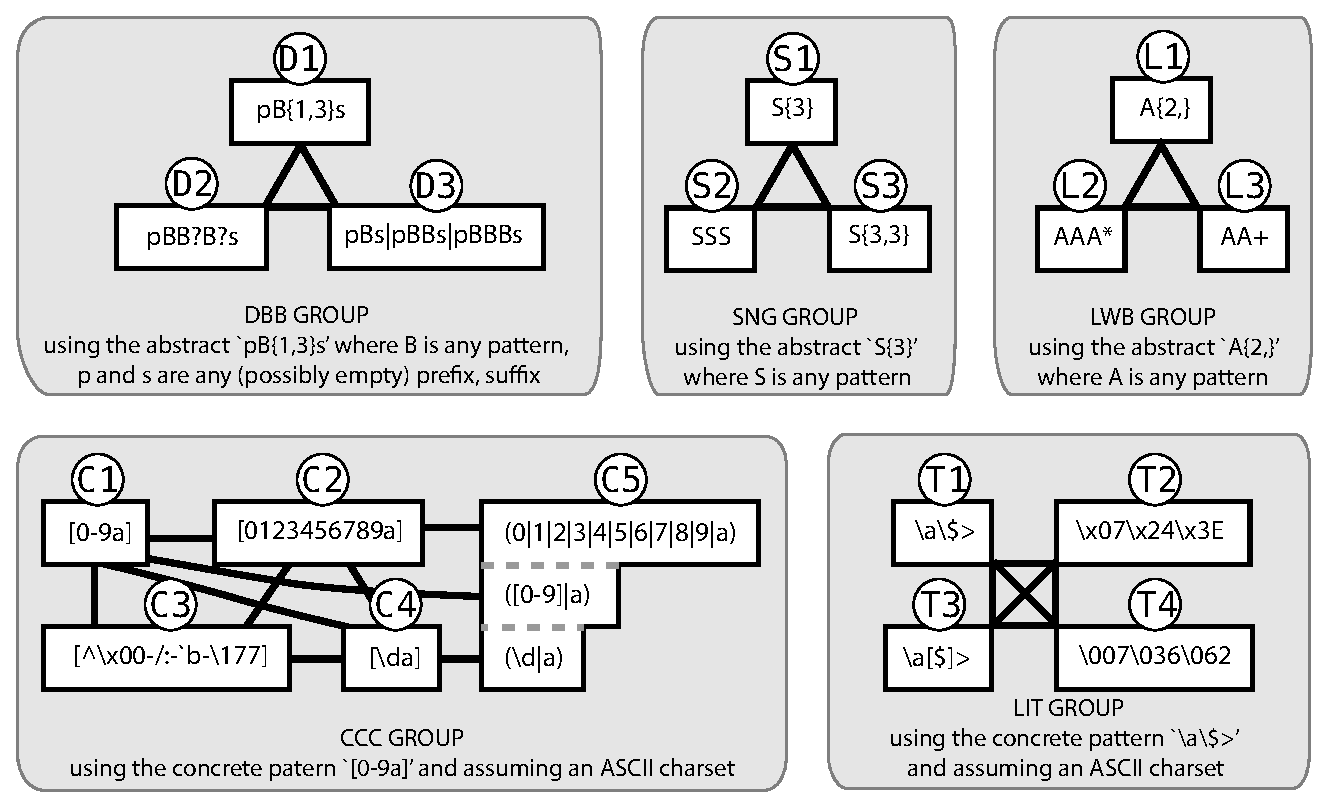
\includegraphics[width=\textwidth]{refactoring/illustrations/refactoringTree.eps}
\vspace{-12pt}
\caption{Equivalence classes with various representations of semantically equivalent refactorings within each class. DBB = Double-Bounded, SNG = Single Bounded, LWB = Lower Bounded, CCC = Custom Character Class and LIT = Literal}
\vspace{-6pt}
\label{fig:refactoringTree}
\end{figure*}




%\footnote{same dataset used in prior work~\cite{chapman2016}}
\section{Refactorings}
\label{sec:refactoring}
After studying over 13,000 distinct regex strings from nearly 4,000 Python projects, we have defined a set of equivalence classes for regexes with refactorings that can transform among members in the classes.
For example,  \verb!AAA*! and \verb!AA+! are semantically identical, except one uses the star operator (indicating zero or more repetitions) and the other uses the plus operator (indicating one or more repetitions).
Both match strings with two or more \verb!A!'s.

Figure~\ref{fig:refactoringTree} displays the five equivalence classes in grey boxes and various semantically equivalent \emph{representations} of a regex are shown in white boxes. For example, LWB is an equivalence class with representations that all have a lower bound on repetitions. Regexes \verb!AAA*! and \verb!AA+!  are both members of this class mapping to representations L2 and L3, respectively, along with the L1 representation, \verb!A{2,}!.
The undirected edges between the representations define possible refactorings.
Identifying the best direction for each arrow in the possible refactorings is discussed in Section~\ref{sec:results}.

We use concrete regexes in the representations to more clearly illustrate examples of the representations. However, the \verb!A!'s in the LWB group abstractly represent any pattern that could be operated on by a repetition modifier (literal characters, character classes, groups, etc.).   We chose the lower bound repetition threshold of  2 for illustration; in practice this could be any number, including zero.
Next, we describe each group, the representations, and possible transformations in detail:

\paragraph{CCC Group}
The Custom Character Class (CCC) group has regex representations that use the custom character class language feature or can be represented by such a feature.
%The character class regex language feature is a fundamental feature found in all language flavors since GREP (check this?).
 A custom character class enables a programmer to specify a set of alternative characters, any of which can match.  For example, the regex \verb!`c[ao]t'! will match both the string ``cat" and the string ``cot" because, between the \verb!c! and \verb!t!, there is a custom character class, \verb![ao]!, that specifies either \verb!a! or \verb!o! (but not both) must be selected.  We use the term \emph{custom} to differentiate these classes created by the user from the default character classes, : \verb!\d!, \verb!\D!, \verb!\w!, \verb!\W!, \verb!\s!, \verb!\S! and \verb!.!,  provided by most regex libraries.
 % For the purposes of our analysis, a negated custom character class (like \verb![^abc]!) is handled separately.
Next, we provide descriptions of each representation in this equivalence class:

\begin{description}  \itemsep -1pt
\item[C1:] Any pattern using a range feature like \verb![a-f]! as shorthand for all of the characters between `a' and `f' (inclusive) within a (non-negative) character class belongs to the C1 node.

\item[C2:] Any pattern that contains at least one (non-negative) custom character class  without any shorthand representations, specifically ranges or defaults. For example, \verb!`[012]'! is in C2, but \verb!`[0-2]'! is not.

\item[C3:] Any character classes expressed using negation, which is indicated by a caret (i.e., \verb!^!) followed by a custom character class specification.
% (including literal characters, default character classes and ranges).
For example, the pattern \verb![^ao]! matches every character \emph{except} \verb!a! or \verb!o!.  If the applicable character set is known (e.g., ASCII, UTF-8, etc.), then any non-negative character class can be represented as a negative character class.  For example, assuming an ASCII charset that has 128 characters: \verb!\x00-\x7f!, a character class representing the lower half: \verb![\x00-\x3f]! can be represented by negating the upper half: \verb![^\x40-\x7f]!.


\item[C4:] Any pattern using a default character class such as \verb!\d! or \verb!\W! within a (non-negative) character class belongs to the C4 node.

\item[C5:] While not expressed using a character class, these representations can be transformed into custom character classes by removing the ORs and adding square brackets (e.g., \verb!(\d|a)! in C5 is equivalent to \verb![\da]! in C4). All custom character classes expressed as an OR of length-one sequences, including defaults or other CCCs, are included in C5. Note that because an OR cannot be directly negated, it does not make sense to have an edge between C3 and C5 in Figure~\ref{fig:refactoringTree}, though C3 may be able to transition to C1, C2 or C4 first and then to C5.
\end{description}

A pattern can belong to multiple representations. For example,  \verb![a-f\d]! belongs to both C1 and C4.  The edge between C1 and C4 represents the opportunity to express the same pattern as \verb![a-f0-9]! by transforming the default digit character class into a range.  This transformed version would only belong to the C1 node.
%\todoNow{add a thing}

\paragraph{DBB Group}
The Double-Bounded (DBB) group contains all regex patterns that use some repetition defined by a (non-equal) lower and upper boundary.  For example the pattern \verb!pB{1,3}s! represents a \verb!p! followed by one to three sequential \verb!B! patterns, then followed by a single \verb!s!.  This will match ``pBs", ``pBBs", and ``pBBBs".

\begin{description}  \itemsep -1pt
\item[D1:] Any pattern that  uses the curly brace repetition with a lower and upper bound, such as  \verb!pB{1,3}s!, belongs to the D1 node.
Note that  \verb!pB{1,3}s! can become \verb!pBB{0,2}s! by pulling the lower bound out of the curly braces and into the explicit sequence (or visa versa). Nonetheless, it would still be part of D1, though this within-node refactoring on D1 is not discussed in this work.
\item[D2:] Any pattern that uses the questionable (i.e., \verb!?!) modifier implies a lower-bound of zero and an upper-bound of one, and belongs to D2. For example, when a double-bounded regex has zero on the lower bound, as is the case with \verb!pBB{0,2}s!  in D1, transforming it to D2 involves replacing the curly braces with $n$ questionable modifiers, where $n$ is the upper bound,  creating \verb!pBB?B?s!.
\item[D3:] Any pattern that has a repetition with a lower and upper boundary and is expressed using ORs is part of D3.  The example, \verb!pB{1,3}s! would become \verb!pBs|pBBs|pBBs! by expanding on each option in the boundaries.
Note also that a pattern can belong to multiple nodes in the DBB group, for example, \verb!(a|aa)X?Y{2,4}! belongs to all three nodes.
% =======
% \item[D1:] Any pattern that  uses the curly brace repetition with a lower and upper bound where the upper and lower bounds are different, such as  \verb!pB{1,3}s!, belongs to the D1 node.
% Note that  \verb!pB{1,3}s! can become \verb!pBB{0,2}s! by pulling the lower bound out of the curly braces and into the explicit sequence (or visa versa). Nonetheless, it would still be part of D1, though this within-node refactoring on D1 is not discussed in this work.
% \item[D2:] Any pattern that uses the questionable (i.e., \verb!?!) modifier implies a lower-bound of zero and an upper-bound of one, and belongs to D2. For example, when a double-bounded regex has zero on the lower bound, as is the case with \verb!pBB{0,2}s!  in D1, transforming it to D2 involves replacing the curly braces with $n$ questionable modifiers, where $n$ is the upper bound,  creating \verb!pBB?B?s!.
% \item[D3:] Any pattern that has a repetition with a lower and upper boundary and is expressed using ORs is part of D3.  The example, \verb!pB{1,3}s! would become \verb!pBs|pBBs|pBBS! by expanding on each option in the boundaries. The challenge with identifying membership in this node is recognizing the opportunity to replace the ORs with double-boundaries, which we discuss in Section~\ref{}.
% >>>>>>> 741a48d7abdf9c0f0b7741ca9a47fda9903c3a0f

%\todoNow{make sure to differentiate this clearly from C5}
\end{description}

Note that a pattern can belong to multiple nodes in the DBB group, for example, \verb!(a|aa)X?Y{2,4}! belongs to all three nodes: \verb!Y{2,4}! maps it to D1, \verb!X?!  maps it to D2, and \verb!(a|aa)!  maps it to D3.

% The same functional pattern can be represented as \verb!lol(ol)?(ol)?!, because the questionable (QST) modifier is used.  Note how in general, this procedure is simply pulling out N QST groups from a curly brace style repetition with a zero lower bound and an upper bound of N.  One question mark is equivalent to the curly brace style with a lower bound of 0, and upper bound of 1, so \verb!X?! is equivalent to \verb!X{0,1}!, so we can express \verb!X{0,2}! as \verb!X?X?!.  Any regex using the QST modifier belongs to the D2 node.



\paragraph{LIT Group}
All patterns that are not purely default character classes have to use some literal tokens to specify what characters to match.  In Python and most other languages that support regex libraries, the programmer is able to specify literal tokens in a variety of ways.  In our example we use the ASCII charset, in which all characters can be expressed using hex and octal codes like \verb!\xF1!, and \verb!\0108!, respectively.  This group defines transformations among various representations of literals.

%Although not all characters can be expressed directly using literal characters typed on the keyboard, the overwhelming majority of patterns do not belong to nodes T2, T3 or T4 because they do not use any of those special features, and so these nodes


\begin{description}  \itemsep -1pt
\item[T1:] Patterns that do not use any hex characters (T2), wrapped characters (T3) or octal (T4), but use at least one literal character belong to the T1 node.
\item[T2:] Any pattern using hex tokens, such as \verb!\x07!, belongs to the T2 node.
\item[T3:]  Any literal wrapped in square brackets belongs to T3.
Literal character can be wrapped in brackets to form a custom character class of size one, such as \verb![x][y][z]!. This style is used most often to avoid using a backslash for a special character in the regex language, for example, \verb![{]! which must otherwise be escaped like \verb!\{!.

\item[T4:] Any pattern using octal tokens, such as \verb!\007!, belongs to the T4 node.
\end{description}

Patterns often fall in multiple of these representations, for example, \verb!abc\007! includes literals \verb!a!, \verb!b!, and \verb!c!, and also octal \verb!\007!, thus belonging to T1 and T4.

\paragraph{LWB Group}
The lower-bounded (LWB) group contains all patterns that specify only a lower boundary on the number of repetitions required for a match.  This can be expressed using curly braces with a comma after the lower bound but no upper bound, for example \verb!A{3,}! which will match `AAA', `AAAA', `AAAAA', and any number of A's greater or equal to 3.


\begin{description}  \itemsep -1pt
\item[L1:] Any pattern using this curly braces-style LWB repetition belongs to node L1.
\item[L2:] The kleene star (KLE) means zero-or-more of something, and so \verb!X*! is equivalent to \verb!X{0,}!.  Any pattern using KLE belongs to the L2 node.
\item[L3:] One of the most commonly used regex features is additional repetition (ADD), for example \verb!T+! which means one-or-more T's.  This is equivalent to \verb!T{1,}!.  Any pattern using ADD repetition belongs to the L3 node.
\end{description}

Regex patterns often belong to multiple nodes, for example, with \verb!A+B*!,  \verb!A+! maps it to L3 and \verb!B*! maps it to L2. We note that the refactorings from L1 to L3 and L2 to L3 are not always possible, specifically when the lower bound is zero and the pattern is not repeated in sequence (e.g., \verb!`A*'! or \verb!`A{0,}'!).

\paragraph{SNG Group} This equivalence class contains  three representations of a regex that  deal with repetition of a single element in the regex, represents by \verb!S!.

\begin{description}  \itemsep -1pt
\item[S1:] Any pattern with a single repetition boundary in curly braces belongs to S1. For example,   \verb!S{3}!, states that S appears exactly three times in sequence.
\item[S2:] Any pattern that is explicitly repeated two or more times and could use repetition operators is part of S2.
\item[S3:] Any pattern with a double-bound in which the upper and lower bounds are same belong to S3. For example, \verb!S{3,3}! states \verb!S! appears a minimum of 3 and maximum of 3 times.
\end{description}

The important factor distinguishing this group from DBB and LWB is that there is a single finite number of repetitions, rather than a bounded range on the number of repetitions (DBB) or a lower bound on the number of repetitions (LWB).

\paragraph{Example}
Regular expressions will often belong to many representations in the equivalence classes described here, and often multiple representations within an equivalence class.
Using an example from a Python project, the regex \verb!`[^ ]*\.[A-Z]{3}'! is a member of S1, L2, C1, C3, and T1. This is because \verb!`[^ ]'! maps it to C3, \verb!`[^ ]*'! maps it to L2, \verb!`[A-Z]'! maps it to C1, \verb!`\.'! maps it to T1, and \verb!`[A-Z]{3}'! maps it to S1.
As examples of refactorings, moving from S1 to S2 would be possible by replacing  \verb!`[A-Z]{3}'! with  \verb!`[A-Z][A-Z][A-Z]'! and moving from L2 to L1 would replace \verb!`[^ ]*'! with \verb!`[^ ]{0,}'!, resulting in a refactored regex of:  \verb!`[^ ]{0,}\.[A-Z][A-Z][A-Z]'!.

% and could be refactored to \emph{S3} as \verb!`[^ ]*\.[A-Z]{3,3}'!  or to \emph{S2} as \verb!`[^ ]*\.[A-Z][A-Z][A-Z]'!, depending on programmer preferences.
%\todoNow{can we have examples from Python projects for all the groups???}







\section{Research Questions}
\label{sec:study}
After defining the equivalence classes and potential  regex refactorings as described in Section~\ref{sec:refactoring}, we wanted to know which representations in the equivalence classes  are considered desirable and which might be smelly. Desirability for regexes can be defined many ways, including maintainable,  understandable, and performance.
%As prior work has shown that regexes are difficult to read~\cite{},
We focus on refactoring for understandability.

We define understandability two ways. First, assuming that common programming practices are more understandable than uncommon practices, we explore the frequencies of each representation from Figure~\ref{fig:refactoringTree} using thousands of regexes scraped from Python projects. Second, we then present people with regexes exemplifying some of the more common characteristics and ask them comprehension questions along two directions: determine which of a list of strings are matched by the regex, and compose a string that is matched by the regex. Our  research questions are:

\begin{description}
\item[RQ1:] Which refactorings have the strongest \emph{community support} based on how frequently each representation appears in regexes in open source Python projects?
\item[RQ2:] Which refactorings have the strongest support based on \emph{understandability} as measured by matching strings and composing strings?
\item[RQ3:] Which regex representations are most desirable based on both community support and understandability?
\end{description}

Next, we present the analysis and results for each  question in turn, followed by a unified discussion in Section~\ref{sec:discussion}.

%First we define a 'Functional Regex'(FR) as some regex that performs in a specific way.  For many FRs, there are several concrete ways to express a single FR.
%We define a concrete regex(CR) as a regex expressed with a particular pattern String.
%Here is one illustration of these definitions:
%
%\todoNow{create some examples for these terms}
%
%We identified 10 loose groups of FRs, described in this table:
%
%\todoNow{create a table explaining the 10 groups}
%
%For each of these groups we created either two concrete versions of three FRs or three concrete versions of two FRs.
%
%Each of the 10 categories had 6 concrete versions of some FR and so there are 60 CRs.  For each CR, we selected 5 \emph{example strings} designed to test the understanding of the CR.  The idea is that different CRs may have different levels of readability, even when they are representing the same FR.  We define readability as the ability to look at the CR and determine if an \emph{example string} can be matched by it or not.
%
%\todoNow{create some illustration of one matching subtask}
%

\begin{table*}[ht]
\begin{small}\begin{center}
\caption{How frequently is each alternative expression style used?}
\label{table:nodeCount}
\begin{tabular}
{lll@{}rrrr}
Node & Description & Example & nPatterns & \% patterns & nProjects & \% projects \\ 
\toprule[0.16em]
%corpusProjectIDs.size(): 1544
C1 & char class using ranges & \begin{minipage}{1.5in}\begin{verbatim}
'^[1-9][0-9]*$'\end{verbatim}\end{minipage}
 & 2,479 & 18.2\% & 810 & 52.5\%\\
C2 & char class explicitly listing all chars & \begin{minipage}{1.5in}\begin{verbatim}
'[aeiouy]'\end{verbatim}\end{minipage}
 & 1,903 & 14.0\% & 715 & 46.3\%\\
C3 & any negated char class & \begin{minipage}{1.5in}\begin{verbatim}
'[^A-Za-z0-9.]+'\end{verbatim}\end{minipage}
 & 1,935 & 14.2\% & 776 & 50.3\%\\
C4 & char class using defaults & \begin{minipage}{1.5in}\begin{verbatim}
'[-+\d.]'\end{verbatim}\end{minipage}
 & 840 & 6.2\% & 414 & 26.8\%\\
C5 & an OR of length-one sub-patterns & \begin{minipage}{1.5in}\begin{verbatim}
'(@|<|>|-|!)'\end{verbatim}\end{minipage}
 & 245 & 1.8\% & 239 & 15.5\%\\
\midrule
D1 & curly brace repetition like \{M,N\} with M<N & \begin{minipage}{1.5in}\begin{verbatim}
'^x{1,4}$'\end{verbatim}\end{minipage}
 & 346 & 2.5\% & 234 & 15.2\%\\
D2 & zero-or-one repetition using question mark & \begin{minipage}{1.5in}\begin{verbatim}
'^http(s)?://'\end{verbatim}\end{minipage}
 & 1,871 & 13.8\% & 646 & 41.8\%\\
D3 & repetition expressed using an OR & \begin{minipage}{1.5in}\begin{verbatim}
'^(Q|QQ)\<(.+)\>$'\end{verbatim}\end{minipage}
 & 10 & .1\% & 27 & 1.7\%\\
\midrule
T1 & no HEX, OCT or char-class-wrapped literals & \begin{minipage}{1.5in}\begin{verbatim}
'get_tag'\end{verbatim}\end{minipage}
 & 12,482 & 91.8\% & 1,485 & 96.2\%\\
T2 & has HEX literal like \verb!\xF5! & \begin{minipage}{1.5in}\begin{verbatim}
'[\x80-\xff]'\end{verbatim}\end{minipage}
 & 479 & 3.5\% & 243 & 15.7\%\\
T3 & has char-class-wrapped literals like [\$] & \begin{minipage}{1.5in}\begin{verbatim}
'[$][{]\d+:([^}]+)[}]'\end{verbatim}\end{minipage}
 & 307 & 2.3\% & 268 & 17.4\%\\
T4 & has OCT literal like \verb!\0177! & \begin{minipage}{1.5in}\begin{verbatim}
'[\041-\176]+:$'\end{verbatim}\end{minipage}
 & 14 & .1\% & 37 & 2.4\%\\
\midrule
L1 & curly brace repetition like \{M,\} & \begin{minipage}{1.5in}\begin{verbatim}
'(DN)[0-9]{4,}'\end{verbatim}\end{minipage}
 & 91 & .7\% & 166 & 10.8\%\\
L2 & zero-or-more repetition using kleene star & \begin{minipage}{1.5in}\begin{verbatim}
'\s*(#.*)?$'\end{verbatim}\end{minipage}
 & 6,017 & 44.3\% & 1,097 & 71.0\%\\
L3 & one-or-more repetition using plus & \begin{minipage}{1.5in}\begin{verbatim}
'[A-Z][a-z]+'\end{verbatim}\end{minipage}
 & 6,003 & 44.1\% & 1,207 & 78.2\%\\
\midrule
S1 & curly brace repetition like \{M\} & \begin{minipage}{1.5in}\begin{verbatim}
'^[a-f0-9]{40}$'\end{verbatim}\end{minipage}
 & 581 & 4.3\% & 340 & 22.0\%\\
S2 & explicit sequential repetition & \begin{minipage}{1.5in}\begin{verbatim}
'ff:ff:ff:ff:ff:ff'\end{verbatim}\end{minipage}
 & 3,378 & 24.8\% & 861 & 55.8\%\\
S3 & curly brace repetition like \{M,M\} & \begin{minipage}{1.5in}\begin{verbatim}
'U[\dA-F]{5,5}'\end{verbatim}\end{minipage}
 & 27 & .2\% & 32 & 2.1\%\\
\bottomrule[0.13em]
\end{tabular}
\end{center}\end{small}\end{table*}




\section{Community Support Study (RQ1)}
\label{communitystudy}
The goal of this study is to understand how frequently each of the regex representations appears in source code. Based on the results, we identify preferred representations using popularity in source code.



\subsection{Artifacts}
To determine how common each regex representations is in the wild, we collected
regexes from GitHub projects. We specifically targeted Python projects as it is a popular programming language with a strong presence on GitHub. Further, Python is the fourth most common language on GitHub (after Java, Javascript and Ruby) and Python's regex pattern
language is close enough to other regex libraries that our conclusions are likely to generalize.

We collected and analyzed static invocations to the Python {\tt re} library.
Figure~\ref{fig:exampleUsage} presents an example  from Python  with key components labeled. The \emph{function} called is {\tt re.compile}.
The \emph{pattern} defines what strings will be matched and the \emph{flag} {\tt re.MULTILINE} modifies the rules used by the regex engine when matching.
When executed, a regex object {\tt r1} is created
%The regex pattern is an ordered series of regular expression language feature tokens.
and it will  match if it finds a zero at the end of a line, or a (possibly negative) integer at the end of a line (i.e., due to the {\tt -?} sequence denoting zero or one instance of the {\tt -}).

\begin{figure}[tb]
\centering
\includegraphics[width=\columnwidth]{refactoring/illustrations/exampleUsage.eps}
\vspace{-12pt}
\caption{Example of one regex library invocation}
\vspace{-6pt}
\label{fig:exampleUsage}
\end{figure}

Our goal was to collect regex patterns from a variety of projects to represent the breadth of how developers use regexes.
We scraped 3,898 projects containing Python code using the GitHub API. This was done by systematically selecting repository IDs, checking the repository for Python files, and retaining the project if Python was found. After dividing eight million repository IDs into 32 groups, we scanned from the beginning until we had collected approximately four thousand Python projects.
%We did so  by dividing a range of about 8 million repo IDs
%into 32 sections of equal size and scanning  for Python projects from the beginning of those
%segments until we ran out of memory.
At that point, we felt we had enough data
to do an analysis without further perfecting our mining techniques.

To identify invocations of the {\tt re} module, we built
the AST of each Python file in each project. In most projects, almost all {\tt re} invocations are present in the
most recent version of a project, but to be more thorough, we also scanned up
to 19 earlier versions.
%The number 20 was chosen to try and maximize returns on
%computing resources invested after observing the scanning process in many hours
%of trial scans.
% If the project had fewer than 20 commits, then all commits were scanned.
% The most recent commit was always included, and the spacing between all other chosen commits was determined by dividing the remaining number of commits by 19 (rounding as needed).
All regex patterns were obtained, sans duplicates.
%Within a project, a duplicate utilization was marked when two versions of the same file have the same function, pattern and flags.
In the end, we observed and recorded 16,088 non-duplicate patterns in 1,645 projects.
%\todoLast{1544 may be a white lie...the 13K+ patterns come from 1544 projects, but the 54k utilizations (before pruning) probably come from something like 1900 projects, and that number is somewhere in the git history of tour de source}

In collecting the set of distinct patterns for analysis,  we ignore the 12.7\%  of {\tt re} invocations using flags, which can alter regex behavior.  An additional 6.5\% of {\tt re} invocations contained patterns that could not be compiled because the pattern was non-static (e.g., used some runtime variable).
%The remaining 80.8\% (43,525) of the utilizations were collapsed into 13,711 distinct pattern strings.
This parser was unable to support 0.8\% (114) due to error.
% of the patterns due to unsupported unicode characters.  Another 0.2\% (25) of the patterns used regex features that we  chose to exclude because they appeared very rarely (e.g., reference conditions).  An additional 0.1\% (16) of the patterns were excluded because they were empty or otherwise malformed so as to cause a parsing error.
After removing all problematic patterns as described and collapsing on duplicates, we ended up with 13,597 distinct patterns from 1,544 projects remained to be used in this study.



\subsection{Metrics}
\label{sec:communitymetric}
We measure community support by matching each regex in the corpus to the representations (nodes) in Figure~\ref{fig:refactoringTree} and counting the number of \emph{patterns} that contain the representation and the number of \emph{projects} that contain the representation.
%A \emph{pattern} is extracted from a utilization, as shown in Figure~\ref{fig:exampleUsage}.
Note that a regex can belong to multiple representations, and a regex can belong to multiple projects since we collapsed duplicates and only analyze the distinct regex patterns.
% that represent 43,525 regex utilizations across the projects.\todoMid{feels weird to hear this again right away, maybe simplify the metrics paragraph}
%For this frequency analysis, we focus on patterns and the number of projects the patterns appear in.
%To determine how often each representation appears in the wild, we extract regex patterns from source code and measure if a representation matches (part of) the pattern.
%
%
%\paragraph{Patterns}



%\paragraph{Projects}

%The process for deciding if a particular pattern belongs to a particular node is described in detail in Section~\ref{communityanalysis}.





\subsection{Analysis}
\label{communityanalysis}
To determine how many of the representations match patterns in the corpus, we performed an analysis using the PCRE parser and by representing the regexes as token streams, depending on the characteristics of the representation. Our analysis code is available on GitHub\footnote{\url{https://github.com/softwarekitty/regex_readability_study}}. Next, we describe the process in detail:

\subsubsection{Presence of a Feature}
For the representations that only require a particular feature to be present, such as the question-mark in D2, the features identified by the PCRE parser were used to decide membership of patterns in nodes.
These feature-requiring nodes are as follows: D1 requires double-bounded repetition with different bounds, D2 requires the question-mark repetition, S1 requires single-bounded repetition, S3 requires double-bounded repetition with the same bounds,  L1 requires a lower-bound repetition, L2 requires the kleene star (\verb!*!) repetition, L3 requires the add (\verb!+!) repetition, and C3 requires a negated custom character class.

\subsubsection{Features  and Pattern}
For some representations, the presence of a feature is not enough to determine membership.
However,  the presence of a feature and properties of the pattern can determine membership.


Identifying D3 requires an OR containing at least two entries - some sequence present in one entry repeated N times, and then the same sequence present in another entry repeated N+1 times.  This is a hard pattern to detect directly, but we identified candidates by looking for a sequence of N repeating groups with an OR-bar (ie. \verb!|!) next to them on one side (either side).  This produced a list of 113 candidates which we narrowed down manually to 10 actual members.


Identifying T2 requires a literal feature that matches the regex \verb!(\\x[a-f0-9A-F]{2})! which reliably identifies hex codes within a pattern.
Similarly T4 requires a literal feature and must match the regex \verb!((\\0\d*)|(\\\d{3}))! which is specific to Python-style octal, requiring either exactly three digits after a slash, or a zero and some other digits after a slash.  Only one false positive was identified which was actually the lower end of a hex range using the literal \verb!\0!.

Identifying T3 requires that a single literal character is wrapped in a custom character class (a member of T3 is always a member of C2).
 T1 requires that no characters are wrapped in brackets or are hex or octal characters, which actually matches over 91\% of the total patterns analyzed.

\subsubsection{Token Stream }
The following representations were identified by representing the regex patterns as a sequence of dot-delimited tokens.
Identifying S2 requires any element to be repeated at least twice. This element could be a character class, a literal, or a collection of things encapsulated in parentheses.
Identifying C1 requires that a non-negative character class contains a range.  Identifying C2 requires that there exists a custom character class that does not use ranges or defaults. Identifying C4 requires the presence of a default character class within a custom character class, specifically, \verb!\d!, \verb!\D!, \verb!\w!, \verb!\W!, \verb!\s!, \verb!\S! and \verb!.!.  Identifying C5 requires an OR of length-one sequences (literal characters or any character class).


\subsection{Results}
Table~\ref{table:nodeCount} presents the frequencies with which each representation appears in a regex pattern and in a project scraped from GitHub. The \emph{node} column references the representations in Figure~\ref{fig:refactoringTree} and the \emph{description} column briefly describes the representation, followed by an \emph{example} from the corpus. The \emph{nPatterns} column counts the patterns that belong to the representation, followed by the percent of patterns out of 13,597.
The \emph{nProjects} column counts the projects that contain a regex belonging to the representation,
followed by the percentage of projects out of 1,544.
Recall that the patterns are all unique and could appear in multiple projects, hence the project support is used to show how pervasive the representation in across the whole community.
For example, 2,479 of the patterns belong to the C1 representation, representing 18.2\% of the patterns. These appear in 810 projects, representing 52.5\%.
 Representation D1 appears in 346 (2.5\%) of the patterns but only 234 (15.2\%) of the projects. In contrast, representation T3 appears in 39 \emph{fewer} patterns but 34 \emph{more} projects, indicating that D1 is more concentrated in a few projects and T3 is more widespread across projects.

Using the pattern frequency as a guide, we can create refactoring recommendations based on community frequency. For example, since C1 is more prevalent than C2, we could say that C2 is smelly since it could better conform to the community standard if expressed as C1. Thus, we might recommend a $\overrightarrow{C2C1}$ refactoring. Based on patterns alone, the winning representations per equivalence class are C1, D2, T1, L2, and S2. With one exception, these are the same for recommendations based on projects. The difference is that L3 appears in more projects than L2, so it is not clear which is more desirable based on community standards.
Section~\ref{sec:rq3} explores these results more deeply.

%Table~\ref{summaryResults} presents these recommendations for each pair of representations within each equivalence class. The \emph{Comm} column is populated based on the findings of \emph{RQ1}. The findings for \emph{RQ2} and \emph{RQ3} are in the \emph{Match} and \emph{Compose} columns, respectively.



\section{Understandability Study (RQ2)}
\label{sec:understandability}
The overall idea of this study  is to present  programmers with one of several representations of semantically equivalent regexes and ask comprehension questions. By comparing the understandability of semantically equivalent regexes that have different representations, we aim to understand which representations  are more desirable and which are more smelly.
This study was  implemented on Amazon's Mechanical Turk with 180 participants.  Each regex pattern was evaluated by 30 participants.
The patterns used were designed to belong to various representations in Figure~\ref{fig:refactoringTree}.



\begin{figure}[tb]
\centering
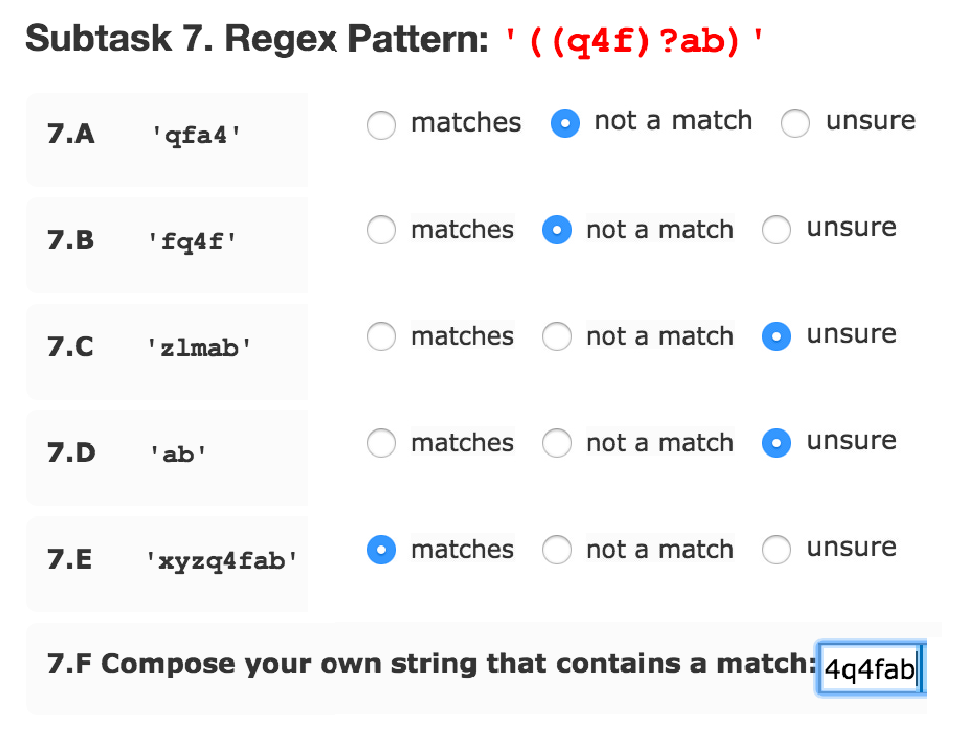
\includegraphics[width=0.8\columnwidth]{refactoring/illustrations/exampleQuestion.eps}
\vspace{-12pt}
\caption{Example of one HIT Question}
\vspace{-6pt}
\label{fig:exampleQuestion}
\end{figure}


\begin{table}
\caption{Matching metric example \label{matchingmetric}}
\begin{center}
\begin{small}
\begin{tabular} {cl | c c c c c}
\textbf{String} & \verb!`RR*'! & \textbf{Oracle} & \textbf{P1} & \textbf{P2} & \textbf{P3}& \textbf{P4}\\ \hline
1 & ``ARROW"    & \checkmark    & \checkmark    & \checkmark    & \checkmark    & \checkmark \\
2 & ``qRs"      & \checkmark    & \checkmark    & \xmark        & \xmark        & ?\\
3 & ``R0R"      & \checkmark    & \checkmark    & \checkmark    & ?             & -\\
4 & ``qrs"      & \xmark        & \checkmark    & \xmark        & \checkmark    & -\\
5 & ``98"       & \xmark        & \xmark        & \xmark        & \xmark        & -\\
\hline
  & Score       & 1.00          & 0.80          & 0.80          & 0.50          & 1.00\\
\\
\multicolumn{7}{l}{\checkmark = match, \xmark = not a match, ? = unsure, -- = left blank}\\
\end{tabular}
\end{small}
\end{center}
\end{table}





\subsection{Metrics}
\label{sec:understadningmetric}
 We measure the understandability of regexes using two complementary metrics, \emph{matching} and \emph{compostition}.


\textbf{Matching:}
 Given a pattern and a set of strings, a participant determines which strings will be matched by the pattern. There are four possible responses for each string, \emph{matches}, \emph{not a match}, \emph{unsure}, or blank. An example from our study is shown in Figure~\ref{fig:exampleQuestion}.

 The percentage of correct responses, disregarding blanks and unsure responses, is the matching score.
 For example, consider regex pattern \verb!`RR*'! and five strings shown in Table~\ref{matchingmetric}, and the responses from four participants in the \emph{P1}, \emph{P2}, \emph{P3} and \emph{P4} columns.
 The oracle has the first three strings matching since they each contain at least one \verb!R! character. \emph{P1} answers correctly for the first three strings but incorrectly thinks the fourth string matches, so the matching score is $4/5 = 0.80$. \emph{P2} incorrectly thinks that the second string is not a match, so they also score $4/5 = 0.80$.  \emph{P3} marks `unsure' for the third string and so the total number of attempted matching questions is 4 instead of 5. \emph{P3} is incorrect about the second and fourth string, so they score $2/4 = 0.50$.  For \emph{P4}, we only have data for the first and second strings, since the other three are blank.  \emph{P4} marks `unsure' for the second matching question so only one matching question has been attempted, and it was answered correctly so the matching score is $1/1 = 1.00$.

Blanks were incorporated into the metric because questions were occasionally left blank in the study. Unsure responses were provided as an option so not to bias the  results when participants were honestly unsure of the answer. These situations did not occur very frequently. Only 1.1\% of the responses were left blank and only 3.8\% of the responses were marked as unsure.  We refer to a response with all blank or unsure responses as an `NA'. Out of 1800 questions, 1.8\%(32) were NA's (never more than 4 out of 30 per pattern).


\textbf{Composition:}
Given a pattern, a participant composes a string they think it matches. If the participant is accurate and the string indeed is matched by the pattern, then a composition score of 1 is assigned, otherwise 0.  For example, given the pattern \verb!`(q4fab|ab)'! from our study, the string, ``xyzq4fab" matches  and would get a score of 1, and the string, ``acb" does not match and would get a score of 0.

To determine a match, each pattern was compiled using the \emph{java.util.regex} library. A \emph{java.util.regex.Matcher} \verb!m! object was created for each composed string using the compiled pattern.  If \verb!m.find()! returned true, then that composed string was given a score of 1, otherwise it was given a score of 0.



\subsection{Design}
%\todoNow{needs to be updated with respect to no C1,T1 nodes}
This study was implemented on the Amazon's Mechanical Turk (MTurk),  a crowdsourcing platform in which requesters can create human intelligence tasks (HITs) for completion by workers. Each HIT is designed to be completed in a fixed amount of time and workers are compensated with money if their work is satisfactory. Requesters can screen workers by requiring each to complete a qualification test prior to completing any HITs.

\subsubsection{Worker Qualification}
Workers qualified to participate in the study by answering questions regarding some basics of regex knowledge. These questions were multiple-choice and asked the worker to describe what the following patterns mean: \verb!`a+'!, \verb!`(r|z)'!, \verb!`\d'!, \verb!`q*'!, and \verb!`[p-s]'!. To pass the qualification, workers had to answer four of the five questions correctly.

\subsubsection{Tasks}
Using the patterns in the corpus as a guide, we created 60 regex patterns that were grouped into 26 semantic equivalence groups.
These semantic groups were focused on exploring edges in the equivalence classes. In this way, we can draw conclusions about transformations between representations since the regexes evaluated were semantically equivalent.

For example, a  group with regexes \verb!`([0-9]+)\.([0-9]+)'! and  \verb!`(\d+)\.(\d+)'! is intended to evaluate the edge between C1 and C4.
 There were 18 groups with two regexes that target various edges in the equivalence classes.
The other eight semantic groups had three regexes each.
For example, a semantic group with regexes \verb!`((q4f){0,1}ab)'!, \verb!`((q4f)?ab)'!, and \verb!`(q4fab|ab)'! is intended to explore the edges among D1, D2, and D3.


%Using the patterns in the corpus as a guide, we created six metagroups containing three pairs of patterns focusing on:
%\begin{itemize}
%\item S1 vs S2
%\item the digit default character class vs C1
%\item the word default character class vs C1
%\item negated digits and words vs C3, whitespace vs C2
%\item additional vs kleene repetition
%\item wrapping vs escaping literal characters
%\end{itemize}
%and four metagroups containing two triplets of patterns focusing on
%\begin{itemize}
%\item octal vs hex vs literal
%\item D1 vs D2 vs D3
%\item C1 vs C2 vs C5
%\item octal vs literal and C2 vs C5
%\end{itemize}
%
%Each of these 10 metagroups contains 6 strings, resulting in a total of 60 regex patterns.  These patterns are logically partitioned into 26 semantic equivalence groups (18 from pairs, 8 from triples).

For each of the 26 groups of patterns, we created five strings, where at least one matched and at least one did not match. These strings were used to compute the matching metric.

Once all the patterns and matching strings were collected, we created tasks for the MTurk participants as follows:
randomly select a pattern from each of the 10 metagroups. Randomize the order of these 10 patterns, as well as the order of the matching strings for each pattern. After adding a question asking the participant to compose a string that each pattern matches, this creates one task on MTurk.   This process was completed until each of the 60 regexes appeared in 30 HITs, resulting in a total of 180 total unique HITs.
An example of a single regex pattern, the five matching strings and the space for composing a string is shown in Figure~\ref{fig:exampleQuestion}.


\subsubsection{Implementation}
Workers were paid \$3.00 for successfully completing a HIT, and were only allowed to complete  one HIT.  The average completion time for accepted HITs was 682 seconds (11 mins, 22 secs).
%A total of 241 HITs were submitted - of those 55 were rejected.
%, and 6 duplicates were ignored, always using the first accepted submission so as to obtain a value for each of the 180 distinct tasks.
A total of 55 HITs were rejected, and  of those, 48 were rushed through by one person leaving many answers blank, 4 other HITs were also rejected because a worker had submitted more than one HIT, one was rejected for not answering composition sections, and one was rejected because it was missing data for 3 questions.  Rejected HITs were returned to MTurk to be completed by others.


%
%
%
%\begin{figure}[tp]
%\begin{small}
%\fbox{\parbox{\columnwidth}{
%\begin{enumerate}
%\item
%\begin{tabular} {lrr}
%\textbf{What is your gender?} & \textbf{n} & \textbf{\%}\\ \hline
%Male & 149 & 83\%\\
%Female & 27& 15\%\\
%Prefer not to say & 4& 2\%
%\end{tabular}
%\item \textbf{What is your age?} \\
%$\mu = 31$, $\sigma = 9.3$
%
%\item
%
%\begin{tabular} {l |rr}
%\textbf{Education Level?} & \textbf{n} & \textbf{\%}\\ \hline
%High School & 5 & 3\%\\
%Some college, no degree & 46 & 26\%\\
% Associates degree & 14 & 8\%\\
%Bachelors degree & 78 & 43\%\\
%Graduate degree & 37 & 21\%\\
%\end{tabular}
%\item
%\begin{tabular} {lrr}
%\textbf{Familiarity with regexes?} & \textbf{n} & \textbf{\%}\\ \hline
%Not familiar at all & 5 & 3\%\\
%Somewhat not familiar & 16 & 9\%\\
%Not sure & 2 & 1\%\\
%Somewhat familiar & 121 & 67\%\\
%Very familiar & 36 & 20\%\\
%\end{tabular}
%\item \textbf{How many regexes do you compose each year?} \\
%$\mu = 67$, $\sigma = 173$
%\item \textbf{How many regexes (not written by you) do you read each year?} \\
%$\mu = 116$, $\sigma = 275$
%%\item In what contexts do you use regexes? \\
%\end{enumerate}
%}}
%\caption{Participant Profiles, $n=180$ \todoLast{can remove this for space} \label{participantprofile}}
%\end{small}
%\end{figure}
%


\subsection{Participants}

In total, there were 180 participants in the study.
A majority were male (83\%) with an average age of 31. Most had
at least an Associates degree (72\%) and most were at least somewhat familiar with regexes prior to the study (87\%). On average,
participants compose 67 regexes per year with a range of 0 to 1000.
%Participants read more regexes than they write with an average of 116 and a range from 0 to 2000.
%Figure~\ref{participantprofile} summarizes the self-reported participant characteristics from the qualification survey.

\input{refactoring/table/testedEdgesTable}


%\todoNow{in study section present choices about pairwise vs random selection for nodes.}


\subsection{Analysis}
For each of the 180 HITs, we computed a matching and composition score for each of the 10 regexes, using the metrics described in Section~\ref{sec:understadningmetric}. This allowed us to compute and then average 26-30 values for each metric  for each of the 60 regexes (fewer than 30 values were used if all the responses in a matching question were unsure or a combination of blanks and unsure). %Next, we computed average scores for matching and composition per regex.
%\todoLast{Mentioning NAs here?}

Each regex was a member of one of 26 groupings of equivalent regexes.
These groupings allow pairwise comparisons of the metrics values to determine which representation of the regex was most understandable and the direction of a refactoring for understandability.
Among all the groups, we performed 42 pairwise comparisons of the matching and composition scores  (i.e., one comparison for each group of size two and three comparisons within each group of size three).
For example, one group had regexes, \verb!RR*! and \verb!R+!, which  represent a transformation between L2 and L3. The former had an average matching of 86\% and the latter had an average matching of 92\%. The average composition score for the former was 97\% and 100\% for the latter. Thus, the community found \verb!R+! from L3 more understandable.
There were two other pairwise comparisons performed between the L2 and L3 group, using regexes pair \verb!zaa*! and \verb!za+'!, and regexes pair \verb!\..*! and \verb!\.+'!.
Considering all three of these regex pairs, the overall matching average for the regexes belonging to L2 was 0.86 and 0.91 for L3.
The overall composition score for L2 was 0.91 and 0.98 for L3. Thus, the community found L3 to be more understandable than L2, from the perspective of both understandability metrics, suggesting a refactoring from L2 to L3.

This information is presented in summary in Table~\ref{table:testedEdgesTable}, with this specific example appearing in the E3 row. The \emph{Index} column enumerates all the pairwise comparisons evaluated in this experiment, \emph{Representations} lists the two representations, \emph{Pairs} shows how many comparisons were performed, \emph{Match1} gives the overall matching score for the first representation listed, \emph{Match2} gives the overall matching score for the second representation listed, and $H_0: \mu_{match1} = \mu_{match2}$ uses the Mann-Whitney test of means to compare the matching scores, and presents the p-values. The last three columns list the average composition scores for the representations and the p-value, also using the Mann-Whitney test of means.

%60 strings
%42 comparisons
%18@2, 8@3
%
%M6R1 ? group 3, 3 comparisons
%- 1 comparisons
%- 0 strings
%
%M3R0 ? group 3, 3 comparisons
%- 1 comparisons
%- 0 strings
%
%M3R1 ? group 3, 3 comparisons
%- 2 comparisons
%- 1 string
%
%M3R0 ? group 3, 3 comparisons
%- 2 comparisons
%- 1 string
%
%58 strings
%36 comparisons


Although we had 42 pairwise comparisons,  we had to drop six comparisons  due to a design flaw since the patterns performed transformations from multiple equivalence classes. For example, pattern \verb!([\072\073])! is in C2 and T4, and was grouped with pattern \verb!(:|;)! in C5, T1, so it was not clear if any differences in understandability were due to the transformation between C2 and C5, or T4 and T1. However, the third member of the group, \verb!([:;])!, could be compared with both, since it is a member of T1 and C2, so comparing it to \verb!([\072\073])! evaluates the transformation between T1 and T4, and comparing to \verb!(:|;)! evaluates the transformation between C2 and C5. The end result is 36 pairwise comparisons across 14 edges from Figure~\ref{fig:refactoringTree}.

\subsection{Results}
Table~\ref{table:testedEdgesTable} presents the results of the understandability analysis. A horizontal line separates the first three edges from the bottom 11. In E1 through E3, there is a statistically significant difference between the representations for at least one of the metrics considering $\alpha = 0.05$.  These represent the strongest evidence for suggesting the directions of refactoring based on the understandability metrics we defined. Specifically, $\overrightarrow{T4 T1}$, $\overrightarrow{D2 D3}$, and $\overrightarrow{L2 L3}$
are likely to improve understandability.

We note here that participants were able to select \emph{unsure} when they were not sure if a string would be matched by a pattern (Figure~\ref{fig:exampleQuestion}). From a comprehension perspective, this indicates some level of confusion and is worth exploring.
% and we can use that to further corroborate the understandability analysis.

%\begin{table*}
%\centering
%\caption{Average Unsure Responses Per Pattern By Node (fewer unsures on the left)}\label{table:unsureResults}
%\begin{tabular}{|| l || cccc || cccc || || cccc || cccc ||}
%                & \multicolumn{4}{c||}{>=Q0(0.67)}         & \multicolumn{4}{c||||}{>=Q1(1.25)}   & \multicolumn{4}{c||}{>=Q2(1.94)}    &  \multicolumn{4}{c||}{>=Q3(2.54)}  \\ \hline
%Node     & L3 & D3 & C2 & C1 & L2 & S2 & S1 & C4 & D1 & C5 & C3 & D2 & T1 & T3 & T2 & T4 \\
%% Number of Patterns - reversed & 4 & 2 & 3 & 3 & 2 & 2 & 4 & 2 & 9 & 3 & 3 & 3 & 8 & 5 & 2 & 3\\
%Unsure Responses Per Pattern & 0.7 & 1 & 1 & 1 & 1.3 & 1.7 & 1.7 & 1.9 & 2 & 2 & 2 & 2.5 & 2.7 & 2.7 & 5.5 & 8.5\\
%\end{tabular}
%\end{table*}

For each pattern, we counted the number of responses containing at least one unsure, representing confusion.
We then grouped the patterns into their representation nodes and computed an average of unsures per pattern.
A higher number may indicate difficulty in comprehending a pattern from that node.
Overall, the highest number of unsure responses came from T4 and T2, which present octal and hex representations of characters. The least number of unsure responses were in L3 and D3.
%, which are both shown to be understandable by looking at E2 and E3 in Table~\ref{table:testedEdgesTable}.
%These nodes and their average number of unsure responses are organized by quartile in Table~\ref{table:unsureResults}.
These results also corroborate the refactorings suggested by the understandability analysis for the LIT group (i.e., $\overrightarrow{T4 T1}$), the DBB group (i.e.,  $\overrightarrow{D2 D3}$), and the LWB group (i.e., $\overrightarrow{L2 L3}$) because the more understandable node has the least unsures of its group.
% The findings for D3 and D2 are contradictory, however, as  and further study is needed.
%  and the number of unsures may be too small to indicate anything, except for T2 and T4.  The one pattern from T4 that had the most unsures of any pattern (i.e., 10 out of 30) was \verb!`xyz[\0133-\0140]'!, so this may have been the least understandable pattern that we tested.





\section{Desirable Representations (RQ3)}
\label{sec:rq3}
To determine the overall trends in the data, we created total orderings on the representation nodes in each equivalence class (Figure~\ref{fig:refactoringTree})  with respect to the community standards (RQ1)  and understandability (RQ2) metrics.

\subsection{Analysis}
At a high level, these total orderings were achieved by building directed graphs with the representations as nodes and edge directions determined by the metrics: patterns and projects for community standards and matching and composition for understandability. Then, within each graph, we performed a topological sort to obtain total node orderings.

The graphs for community support are based on Table~\ref{table:nodeCount} and the graphs for understandability are based on Table~\ref{table:testedEdgesTable}. The following sections describe the processes for building and and topologically sorting the graphs.

\begin{figure}[tb]
\centering
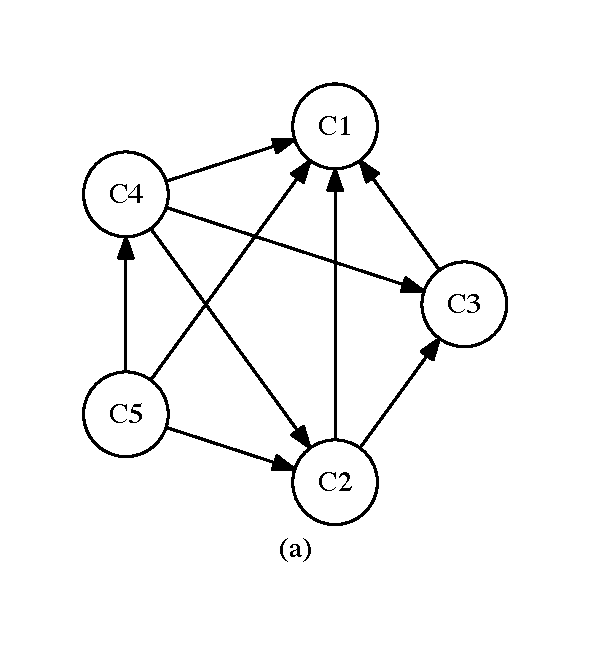
\includegraphics[width=0.42\columnwidth]{refactoring/graphs/cart.pdf}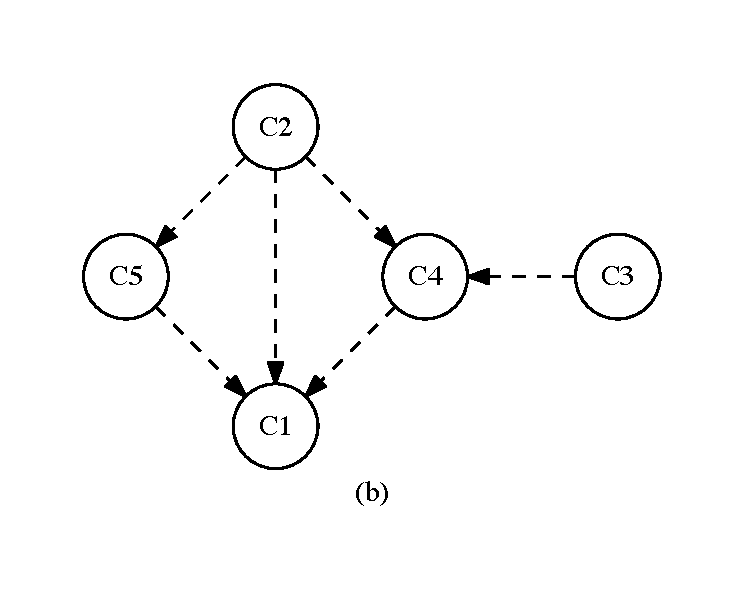
\includegraphics[width=0.57\columnwidth]{refactoring/graphs/ccom.pdf}
\vspace{-12pt}
\caption{Trend graphs for the CCC equivalence graph: (a) represent the artifact analysis, (b) represent the understandability analysis.}

\label{fig:graphsforanalysis}
\end{figure}

\subsubsection{Building the Graphs}
In the community standards graph, we represent a directed edge  $\overrightarrow{C2  C1}$ when  nPatterns(C1) $>$ nPatterns(C2) \emph{and}  nProjects(C1) $>$ nProjects(C2).
When there is a conflict between nPatterns and nProjects, as is the case between L2 and L3 where L2 is found in more patterns and L3 is found in more projects, an undirected edge $\overline{L2L3}$ is used.
This represents that there was no winner based on the two metrics.
After considering all pairs of nodes in each equivalence class that also have an edge in Figure~\ref{fig:refactoringTree}, we have created a graph, for example Figure~\ref{fig:graphsforanalysis}a, that represents the frequency trends among the community artifacts.
%Note that with the CCC group, there is no edge between C3 and C5 because there is no straightforward refactoring between those representations, as discussed in Section~\ref{sec:refactoring}.

In the understandability graph, we represent a directed edge  $\overrightarrow{C2C1}$ when match(C1) $>$ match(C2) \emph{and} compose(C1) $>$ compose(C2). When there is a conflict between match and compose, as is the case with T1 and T3 where match(T1) is higher but compose(T3) is higher, an undirected edge $\overline{T1T3}$ is used. When one metric has a tie, as is the case with composition in E9, we resort to the matching metric to determine  $\overrightarrow{C5C1}$. An example understandability graph for the CCC is shown in Figure~\ref{fig:graphsforanalysis}b.
%\footnote{When there are confounded representations, as is the case with E8, E4, and E5 which all use tranformations from the CCC and the LIT equivalence classes, we omit those from the understandability graph. This makes sense since all use a transformation between T1 and T4 strongly favoring T1. }

\subsubsection{Topological Sorting}
Once the graphs are built for each equivalence class and each set of metrics, community standards and understandability, we apply a modified version of Kahn's topological sorting algorithm to obtain a total ordering on the nodes, as shown in Algorithm~\ref{topological}. The first modification is to remove all undirected edges since Kahn's operates over a directed graph.

In Kahn's algorithm, all nodes without incoming edges are added to a set $S$ (Line~\ref{addnoincomingtos}), which represents the order in which nodes are explored in the graph. For each $n$ node in $S$ (Line~\ref{beginwhile}), all edges from $n$ are removed and $n$ is added to the topologically sorted list $L$ (Line~\ref{addntoL}). If there exists a node $m$ that has no incoming edges, it is added to $S$.  In the end, $L$ is a topologically sorted list.

\begin{algorithm}
  \caption{Modified Topological Sort}\label{topological}
  \begin{algorithmic}[1]
\State  $L \gets$ []
\State $S \gets$ []
\State Remove all undirected edges (creates a DAG)
\State Add all disconnected nodes to $L$ and remove from graph. If there is more than one, mark the tie. \label{markTie1}
\State Add all nodes with no incoming edges to $S$. If there is more than one, mark the tie. \label{addnoincomingtos}
\While {$S$ is non-empty} \label{beginwhile}
	\State remove a node $n$ from $S$ \label{setn}
	\State add $n$ to $L$  \label{addntoL}
	\For {node $m$ such that $e$ is an edge $\overrightarrow{nm}$}
		\State remove $e$
		\If{$m$ has no incoming edges}
			\State add $m$ to $S$ \label{addToS}
		\EndIf
	\EndFor
	\State If multiple nodes were added to $S$ in this iteration, mark the tie \label{markTie2}
	\State remove $n$ from graph
\EndWhile
\State For all ties in $L$, use a tiebreaker.
  \end{algorithmic}
\end{algorithm}

One downside to Kahn's algorithm is that the total ordering is not unique. Thus, we mark ties in order to identify when a tiebreaker is needed to enforce a total ordering on the nodes. For example, on the understandability graph in Figure~\ref{fig:graphsforanalysis}b, there is a tie between C3 and C2 since both have no incoming edges, so they are marked as a tie on Line~\ref{addnoincomingtos}. Further, when $n=C2$ on line~\ref{setn}, both C5 and C4 are added to $S$ on Line~\ref{addToS}, thus the tie between them is marked on line~\ref{markTie2}. In these cases, a tiebreaker is needed.

Breaking ties on the community standards graph involves choosing the representation that appears in a larger number of projects, as it is more widespread across the community.

Breaking ties in the understandability graph uses the metrics. Based on Table~\ref{table:testedEdgesTable}, we compute the average matching score for all instances of each representation, and do the same for the composition score. For example, C4 appears in E5, E12 and E13 with an overall average matching score of 0.81 and composition score of 24.3. C5 appears in E4 and E9 with an average matching of 0.87 and composition of 28.28. Thus, C5 is favored to C4 and appears higher in the sorting.

\subsection{Results}
After running the topological sort in Algorithm~\ref{topological} with tiebreakers, we have a total ordering on nodes for each graph, shown in Table~\ref{topologicalResults}.  For example, given the graphs in Figure~\ref{fig:graphsforanalysis}a and Figure~\ref{fig:graphsforanalysis}b, the topological sorts are {\tt C1 C3 C2 C4 C5} and {\tt C1 C5 C4 C2 C3}, respectively.

\begin{table*}
\centering
\caption{Topological Sorting, with the left-most position being highest \label{topologicalResults}}
\begin{tabular}{|| l || l || l || l || l || l ||}
				& CCC			& DBB 		& LBW & SNG & LIT \\ \hline
Community Standards		& C1 C3 C2 C4 C5 	& D2 D1 D3	&  L3 L2 L1 	& S2 S1 S3 	& T1 T3 T2 T4 \\
Understandability 			& C1 C5 C4 C2 C3 	& D3 D1 D2 	& L3 L2		& S2 S1		& T1 T2 T4 T3 \\
\end{tabular}
\end{table*}




There is a clear winner in each equivalence class, with the exception of DBB.
That is, the node sorted highest in the topological sorts for both the community standards and understandability analyses are C1 for CCC, L3 for LBW, S2 for SNG, and T1 for LIT.
After the top rank, it is not clear who the second place winner is in any of the classes, however, having a consistent and clear winner is evidence of a preference with respect to community standards and understandability, and thus provides guidance for potential refactorings.

This positive result, that the most popular representation in the corpus is also the most understandable, makes sense as people may be more likely to understand things that are familiar or well documented. However, while L3 is the winner for the LBW group, we note that L2 appears in slightly more patterns.

DBB is different  as the orderings are completely reversed depending on the analysis, so the community standards favor D2 and understandability favors D3. Further study is needed on this, as well as on LBW and SNG since not all nodes were considered in the understandability analysis.







%\begin{table}[t]
%\caption{Summary of Refactoring Directions \label{summaryResults}}
%\begin{center}
%\begin{tabular}{|c@{ }c | c  l l @{}|} \hline
%\multicolumn{2}{|c|}{\textbf{Pair}} & \textbf{Com} & \textbf{Match} & \textbf{Compose} \\ \hline \hline
%C1 & C2 & $\Leftarrow$  & $\Leftarrow$ (E1) $\Rightarrow$ (E2,E3) & $\Leftarrow$ (E1) $\Rightarrow$ (E2,E3)\\
%C1 & C3 & $\Leftarrow$ & & \\
%\textbf{C1} & C4 & $\Leftarrow$ & $\equiv$ (E4) & $\Leftarrow$  (E4)\\
%C1 & C5 & $\Leftarrow$ & $\Leftarrow$ (E5) & $\Rightarrow$ (E5) \\
%C2 & C3 & $\Rightarrow$ & & \\
%C2 & C4 & $\Leftarrow$ & $\Rightarrow$ (E6) & $\Rightarrow$ (E6)\\
%C2 & C5 & $\Leftarrow$ & $\Rightarrow$ (E7,E8) & $\Rightarrow$ (E7,E8)\\
%C3 & C4 & $\Leftarrow$ & & \\
%C3 & C5 & $\Leftarrow$ & & \\
%C4 & C5 & $\Leftarrow$ & & \\
%\hline
%D1 & D2 & $\Rightarrow$ & $\Leftarrow$ (E9)& $\Leftarrow$ (E9) \\
%D1 & \textbf{D3} & $\Rightarrow$ & $\Rightarrow$ (E10)& $\Rightarrow$ (E10) \\
%D2 & D3 & $\Leftarrow$ & $\Rightarrow$ (E11) & $\Rightarrow$ (E11) \\
%\hline
%L1 & L2 & $\Rightarrow$ & & \\
%L1 & L3 & $\Leftarrow$ & & \\
%L2 & L3 & $\Leftarrow$ & $\Rightarrow$ (E12) & $\Rightarrow$ (E12)  \\
%\hline
%S1 & S2 & $\Rightarrow$ & $\Leftarrow$ (E13) & $\Leftarrow$ (E13) \\
%S1 & S3 & $\Leftarrow$ & & \\
%S2 & S3 & $\Leftarrow$ & & \\
%\hline
%\textbf{T1} & T2 & $\Leftarrow$  & $\Leftarrow$ (E2)& $\Leftarrow$ (E2) \\
%T1 & T3 & $\Leftarrow$ & $\Leftarrow$ (E14) & $\Rightarrow$ (E14)\\
%\textbf{T1} & T4 & $\Leftarrow$ & $\Leftarrow$ (E3,E8,E15) & $\Leftarrow$ (E3,E8,E15)\\
%T2 & T3 & $\Leftarrow$ & & \\
%\textbf{T2} & T4 & $\Leftarrow$ & $\Leftarrow$ (E16) & $\Leftarrow$ (E16)\\
%T3 & T4 & $\Leftarrow$ & & \\
%\hline
%%1 & 2 &  & & \\
%%1 & 3 &  & & \\
%%2 & 3 &  & & \\
%
%
%\end{tabular}
%\end{center}
%\end{table}


%\section{Results}
%\label{sec:results}
%
%
%
%
%
%
%\subsection{RQ3: Overlap in Refactorings}
%
%%\begin{figure}[tb]
%%\centering
%%\includegraphics[width=\columnwidth]{illustrations/exampleUsage.eps}
%%\vspace{-12pt}
%%\caption{Example of one regex utilization}
%%\vspace{-6pt}
%%\label{fig:exampleUsage}
%%\end{figure}
%
%
%
%
%
%
%
%
%
%%\paragraph{CCC Group}
%%This group is full of disagreement among the metrics. Five pairs were evaluated by all methods and only one pair, $C1 \Leftarrow C4$, has a somewhat clear winner with C1 (note that the matching metric is equivalent). All the others have disagreement between the community and understandability, or between the understandability metrics, matching and composition.
%%
%%
%%\paragraph{DBB Group}
%%D2 has the most community support appearing in nearly 14\% of the patterns, yet the understandability metrics favor both D1 and D3 over D2. The results are consistent across the board that D3 is always favorable to D1.
%%
%%\paragraph{LWB Group}
%%
%%\paragraph{LIT Group}
%%
%%\paragraph{SNG Group}
%%
%%=======
%%\paragraph{CCC Group}
%%This group is full of disagreement among the metrics. Five pairs were evaluated by all methods and only one pair, $C1 \Leftarrow C4$, has a somewhat clear winner with C1 (note that the matching metric is equivalent). All the others have disagreement between the community and understandability, or between the understandability metrics, matching and composition.
%%
%%
%%\paragraph{DBB Group}
%%D2 has the most community support appearing in nearly 14\% of the patterns, yet the understandability metrics favor both D1 and D3 over D2. The results are consistent across the board that D3 is always favorable to D1.
%%
%%\paragraph{LWB Group}
%%\todoNow{Carl filling in these and adding some observations and context}
%%
%%\paragraph{LIT Group}
%%
%%\paragraph{SNG Group}
%%
%%>>>>>>> 61b90cac1ea534594cd76837430bc23ee51cc916
%
%
%
%
%%
%%(for rough draft...)
%%
%%Looks like M6 and M8 are the best meta-refactorings according to ANOVA.
%%If you peek at MTResults Processing.csv on google docs, M6 has the best refactoring...every OCTAL type should be converted to an OR or preferably a CCC.
%%
%%M8 has a weak P value, but still ok in one case (0.12) and consistently says that 'aa*' should be written as 'a+'.
%%
%%Looks like M0, M1, M2, M3 and M9 are very dependent on the regex chosen, so regex-specific refactorings like:
%%0.1401 \verb!&d([aeiou][aeiou])z'    &d([aeiou]{2})z'!
%%0.075   \verb![\t\r\f\n ]'    [\s]'!
%%0.1024  \verb![a-f]([0-9]+)[a-f]' [a-f](\d+)[a-f]'!
%%0.1271  \verb![\{][\$](\d+[.]\d)[}]'!
%%\verb!\\\{\\\$(\d+\.\d)\}'!
%%(from M0,M1,M2,M9 respectively)
%%
%%have okay P-values and may indicate regex-specific refactorings, but do not indicate an overall trend for that type of refactoring.
%%Notice that M3 does not even have a strong p-value candidate, but this may be thrown off because of the very confusing regex chosen for CCC:
%%0.78    0.79
%%\verb!xyz[_\[\]`\^\\]'!    \verb!xyz[\x5b-\x5f]'!
%%which has a lot of escape characters, so that the hex group was easier to understand than the CCC.
%%
%%
%%
%%Meanwhile M4,M5 and M7 have both ambiguous p-values and anova results.  But this is still a finding: that no refactoring is needed between things like:
%%\verb!(q4fab|ab)'! (\verb!(q4f){0,1}ab)'!
%%\verb!tri[abcdef]3'!   \verb!tri(a|b|c|d|e|f)3'!
%%\verb!&(\w+);'!    \verb!&([A-Za-z0-9_]+);'!
%%(from M4,M5,M7 respectively)
%%
%%Although one refactoring from M5 might be of slight interest:
%%0.1196  FALSE   \verb!tri[a-f]3'!  \verb!tri(a|b|c|d|e|f)3'!
%
%%\todoMid{more data from the composition problems}

%\begin{table}\begin{small}\begin{center}\caption{some Group table caption}\label{table:groupANOVATable}\begin{tabular}
%{lcc}
%group & Pregex & Prefactoring \\
%\toprule[0.16em]
%CCC & <0.001 & 0.261\\
%DBB & 0.591 & 0.072\\
%LIT & 0.002 & 0.639\\
%LWB & 0.990 & 0.041\\
%SNG & <0.001 & 0.958\\
%\bottomrule[0.13em]\end{tabular}\end{center}\end{small}\end{table}

\section{Discussion}
\label{sec:discussion}
Based on our analyses of source code and our empirical study on the understandability of regex representations, we have identified preferred regex representations that may make regexes easier to understand and thus maintain. In this section, we describe the implications of these results.

\subsection{Interpreting Results}
In the CCC equivalence class, C1 (e.g., \verb![0-9a]!) is more commonly found in the patterns and projects.  Representations C2 (e.g., \verb![0123456789a]!) and C3 (e.g., \verb![^\x00-/:-`b-\x7F]!) appear in similar percentages of patterns and projects but there is no significant difference in understandability considering two pairs of regexes tested as part of E13 (Table~\ref{table:testedEdgesTable}). However, a small preference is shown for C1 over C2 (E7), leading this to to be the winner of both the community support and understandability analyses.    Regex length is probably important for understandability, though we did not test for this.

% - the longest regex in the corpus is \todoNow{X} characters long...
%Anyway C2 is comon but less readable.  C4 is somehwat less common to use defalut in CC - why?  C5 is rare, but marginally more readable than C2.  Not enough data or contrast to come to a conclusion about C3 - it is a catch-all?

In the DBB group, D3 (e.g., \verb!pBs|pBBs|pBBBs!) merits further exploration because it is the most understandable but least common node in DBB group.  This may be because explicitly listing the possibilities with an OR is easy to grasp, but if the number of items in the OR is too large, the understandability may go down. Further analysis is needed to determine the optimal thresholds for representing a regex as D3 compared to D1 (e.g., \verb!pB{1,3}s!) or D2 (e.g., \verb!pBB?B?s!).
%Intuitively, it seems that D2 may be more common because 0,1 is just a more common use case than an arbitrary range like 4, 25.

In the SNG group, S1 is a compact representation (e.g., \verb!S{3}!), but S2 was preferred (e.g., \verb!SSS!). Similar to the DBB group, this may be do to the particular examples chosen in the analysis, as a large number of explicit repetitions may not be as preferred.

In the LWB group,  L1 (e.g., \verb!A{2,}!) is rare, appearing in $<1$\% of the patterns. Representations L2 (e.g., \verb!AAA*!) and L3 (e.g., \verb!AA+!) appear in similar numbers of patterns and projects, but there is a significant difference in their understandability, favoring L3.
% , it's clear that this is a rare use case, and also that L3 is the most common  use case.  Patterns using star are secondary, helper patterns because they will trivially match anything, so they are less common.  But anyway...


% is nice, but
%so probably better than S2.  S2 is over-weighted because of double-characters in regular words like foot.
In the LIT group, T1 (e.g., \verb!\a\$>!) is the typical way to list literals, but the reason to use hex (T2) or oct (T4) types is because some characters cannot be represented any other way, like invisible chars.  One main result of our work is that  T4 (e.g., \verb!\007\036\062!) is  less understandable   than T2 (e.g., \verb!\x07\x24\x3E!), so if invisible chars are required, hex is the more understandable representation.
Regarding T3 (e.g., \verb!\a[$]>!), initially we thought the square brackets would be more understandable than using an escape character,  but we found the opposite. Given a choice between T1 and T3, the escape character was more understandable.

\subsection{Opportunities For Future Work}
There are several directions for future work related to regex study and refactoring.

\paragraph{Equivalence Class Models}
We looked at five equivalence classes, each with three to five nodes.
Future work could consider richer models with more or different classes and nodes.
%For example, we have looked at all ranges as equivalent, all defaults as equivalent, and relied on many such generalizations.  However, the range \verb![a-f]! is likely to be more understandable for most people than a range like \verb![:-`]!.
%In addition to breaking our 5 groups into more specific nodes, future work could model refactorings outside of these groups.
%
%We have not determined a list of all possible refactoring groups given the functional variety and significant number of features to consider, but we are aware of a few additional equivalence classes outside of our 5 groups, such as:
Additional equivalence groups to consider may include:
\begin{description} \itemsep -2pt
%\item[Single line option]  \verb!'''(.|\n)+'''! $\equiv$ \verb!(?s)'''(.)+'''!
\item[Multi line option]  \verb!(?m)G\n! $\equiv$ \verb!(?m)G$!
\item[Case insensitive]  \verb!(?i)[a-z]! $\equiv$ \verb![A-Za-z]!
\item[Backreferences]  \verb!(X)q\1! $\equiv$ \verb!(?P<name>X)q\g<name>!
%\item[Word Boundaries]  \verb!\bZ! $\equiv$ \verb!((?<=\w)(?=\W)|(?<=\W)(?=\w))Z!
\end{description}



It might also be the case that there exist critical comprehension differences within a representation. For example, between C1 (e.g., \verb![0-9a]!) and C4 (e.g., \verb![\da]!), it could be the case that \verb![0-9]! is preferred to \verb![\d]!, but \verb![A-Za-z0-9_]! is not be preferred to \verb![\w]!).
By creating a more granular model of equivalence classes, and making sure to carefully evaluate alternative representations of the most frequently used specific patterns,  additional useful refactorings could be identified.


%We focused on refactorings within a group, treating groups as orthogonal to one another.  It would be interesting to see if there is some cooperation between pairs of edges in separate groups by applying more than one type of refactoring at once.

%\paragraph{Understandability}
%
%
%%One of the most straightforward ways to address understandability is to directly ask software professionals which from a list of equivalent regexes they prefer and why.
%% but at least one side of the refactoring was contrived and we did not focus on any specific community (the 1544 projects we obtained regexes from were randomly obtained).
%% If understandability measurements used regexes sampled from the codebase of a specific community(most frequently observed regexes, most buggy regexes, regexes on the hottest execution paths, etc.), and measured the understanding of programming professionals working in that community, then the measurements and the refactorings they imply would be more likely to have a direct and certain positive impact.
%
%In another study, we did a survey where software professionals indicated that understandability of regexes they find in source code is a major pain point.  In this study, our participants indicated that they read about twice as many regexes as they compose.  What is the impact on maintainers, developers and contributors to open-source projects of not being able to understand a regex that they find in the code they are working with?  Presumably this is a frustrating experience - how much does a confusing regex slow down a software professional?  What bugs or other negative factors can be attributed to or associated with regexes that are difficult to understand?  How often does this happen and in what settings?  Future work could tailor an in-depth exploration of the overall costs of confusing regexes and the potential benefits of refactoring or other treatments for confusing regexes.

\paragraph{Regex Migration Libraries}
We have identified opportunities
 to improve the understandability of regexes in existing code bases by looking for some of the less understandable regex representations, which can be thought of as antipatterns, and refactoring to the more common or understandable representations.
 Building migration libraries is a promising direction of future work to ease the manual burden of this process, similar in spirit to prior work on class library migration~\cite{Balaban:2005:RSC:1103845.1094832}.

%\paragraph{Regex Refactoring Applications}
%Maintainers of code that is intentionally obfuscated for security purposes may want to develop regexes that they understand and then automatically transform them into the least understandable regex possible.
%
%One fundamental concept that many users of regex struggle to learn is when to use regexes for simple parsing, and when to write a full-fledged parser (for example, when parsing HTML).  Regexes that are trying to parse HTML, XML or similar languages could be refactored not into a better regex, but into some code with an equivalent intention that does parsing much better.

\paragraph{Regex Programming Standards}
Many organizations enforce coding standards in their repositories to ease understandability.
Presently, we are not aware of coding standards for regular expressions, but this work suggests that enforcing standard representations for various regex constructs could ease comprehension.

\paragraph{Regex Refactoring for Performance}
The representation of regexes may have a strong impact on the runtime performance of a chosen regex engine. Prior work has sought to expedite the processing of regexes over large bodies of text~\cite{Baeza-Yates:1996:FTS:235809.235810}.
Refactoring regexes for performance would complement those efforts.
%Further study is needed to determine which representations are most efficient, leading to a whole new area of study on regex refactoring for performance, a topic already explored for
%Depending on the efficiency of an organization's chosen regex engine, an organization may want to enforce standards for efficiency.
%, or for compatibility with a regex analysis tool like Z3, HAMPI, BRICS or REX.

\subsection{Threats to Validity}

\textbf{Internal}
We measure understandability of regexes using two metrics, matching and composition. However, these measures may not reflect actual understanding of the regex behavior. For this reason, we chose to use two metrics and present the analysis in the context of reading and writing regexes, but the threat remains.

Participants evaluated regular expressions during tasks on MTurk, which may not be representative enough of the context in which programmers would encounter regexes in practive. Further study is needed to determine the impact of the experimentation context on the results.

Some regex representations from the equivalence classes were not involved in the understandability analysis and that may have biased the results against those nodes. Repetition of the analysis with more compete coverage of the edges in the equivalence classes is needed.

We treated unsure responses as omissions that  did not count  against the matching scores. Thus, if a participant answered two strings correctly and marked the other three strings as unsure, then this was 2/2 correct, not 2/5. This may have inflated the matching scores, however, less than 5\% of the matching scores were impacted by such responses.


%
%In our analyses, we measure understandability using matching and composition metrics.
%However, there may be other ways to approach regex understandability, such as deciding which regexes in a set are equivalent, finding the minimum modification to some text so that a given regex will match it.
%It may also be meaningful to provide some code that exists around a regex as context, since that would better represent a scenario in which programmers would encounter regexes in practice.
%Further study is needed to determine if the chosen metrics and experimentation context have resulted in a reasonable measure of understandability.

\textbf{External}
Participants in our survey came from MTurk, which may not be representative of people who read and write regexes on a regular basis.

The regexes  used in the evaluation were inspired by those found in Python code, which is just one language that has library support for regexes. Thus, we may have missed opportunities for other refactorings based on how programmers use regexes in other programming languages.

The results of the understandability analysis may be closely tied to the particular regexes chosen for the experiment. For many of the representations, we had several comparisons. Still, replication with more regex patterns is needed.% to validate our results.

%\todoMid{what about the threat of too few examples per node?  Didn't cover every edge.  Regex set is randomly collected online, not focused on any specific target audience.}

%Our community analysis only focuses on the Python language, but as the vast majority of regex features are shared across most general programming languages (e.g., Java, C, C\#, or Ruby), a Python {pattern} will (almost always) behave the same when used in other languages and our results are likely to generalize.
%, whereas a utilization is not universal in the same way (i.e., it may not compile in other languages, even with small modifications to function and flag names).
%As an example, the {\tt re.MULTILINE} flag, or similar, is present in Python, Java, and C\#, but  the Python {\tt re.DOTALL} flag is not present in C\# though it has an equivalent flag in Java.


\section{Related Work}
\label{sec:related}
Regular expression understandability has not been studied directly, though prior work has suggested that regexes are hard to read and understand since there are tens of thousands of bug reports related to regular expressions~\cite{Spishak:2012:TSR:2318202.2318207}. 
To aid in regex creation and understanding,  tools have been developed to support more robust creation~\cite{Spishak:2012:TSR:2318202.2318207} or to allow visual debugging~\cite{Beck:2014:RVD:2591062.2591111}. Building on the perspective that regexes are difficult to create, other research has focused on removing the human from the creation process by learning regular expressions from  text~\cite{Babbar:2010:CBA:1871840.1871848, Li:2008:REL:1613715.1613719}.

Regular expression refactoring has also not been studied directly, though refactoring literature abounds~\cite{Mens:2004:SSR:972215.972286, Opdyke:1992:ROF:169783, Griswold:1993:AAP:152388.152389}. 
The closest to regex refactoring comes from research toward  expediting the processing of regular expressions on large bodies of text~\cite{Baeza-Yates:1996:FTS:235809.235810}, which could be thought of as refactoring for performance. 

Code smells in object-oriented languages were introduced by Fowler~\cite{Fowl1999}. Researchers have studied the impact of code smells on program comprehension~\cite{abbes2011empirical, du2006does}, finding that the more smells in the code, the harder the comprehension. This is similar to our work, except we aim to identify which  regex representations can be considered smelly. 
Code smells have been extended to other language paradigms including end-user programming languages~\cite{Hermans2012intra, Hermans2012intraExt, stoleeicse, stoleeTSE}. The code smells identified in this work are representations that are not common or not well understood by developers. This concept of using community standards to define smells has been used in other refactoring literature  for end-user programmers~\cite{stoleeicse, stoleeTSE}. 

Exploring language feature usage by mining source code has been studied extensively for
Smalltalk~\cite{Callau:2011:DUD:1985441.1985448},
JavaScript~\cite{Richards:2010:ADB:1809028.1806598},
and Java~\cite{Dyer:2014:MBA:2568225.2568295, Grechanik:2010:EIL:1852786.1852801, Parnin:2013:AUJ:2589712.2589717, Livshits:2005:RAJ:2099708.2099724},
and more specifically,
Java generics~\cite{Parnin:2013:AUJ:2589712.2589717} and
Java reflection~\cite{Livshits:2005:RAJ:2099708.2099724}.
Our prior work (~\cite{chapman2016}, under review) was the first to mine and evaluate regular expression usages from existing software repositories. The intention of the prior work~\cite{chapman2016} was to explore regex language features  usage and surveyed developers about regex usage. In this work, we define potential refactorings and use the mined corpus to find support for the presence of various regex representations in the wild. Beyond that, we measure regex understandability and suggest canonical representations for regexes to enhance conformance to community standards and understandability. 

%Related to mining work, regular expressions have been used to form queries in mining framework~\cite{Begel:2010:CDE:1806799.1806821}, but have not been the focus of the mining activities.
%Surveys have been used to measure adoption of various programming languages~\cite{Meyerovich:2013:EAP:2509136.2509515, Dattero:2004:PLG:962081.962087}, and been combined with  repository analysis~\cite{Meyerovich:2013:EAP:2509136.2509515}, but have not focused on regexes.

%Mining properties of open source repositories is a well-studied topic, focusing, for example, on API usage patterns~\cite{Linares-Vasquez:2014:MEA:2597073.2597085}.

%
%
%
%Refactoring comprehension 
%
%Refactoring for understandability~\cite{6405299, stoleeicse, stoleeTSE} and conformance to the community in end-user programs~\cite{stoleeicse, stoleeTSE}.
%
%
%Regular expression education
%
%
%Focus on language design for a regex extension to Haskell~\cite{Broberg:2004:REP:1016848.1016863}.  
%

%Regular expressions have been a focus point in a variety of research objectives. 
%
%Regarding applications, regular expressions have been used for test case generation~\cite{Ghosh:2013:JAT:2486788.2486925, Galler:2014:STD:2683035.2683100, Anand:2013:OSM:2503903.2503991, Tillmann:2014:TAT:2642937.2642941},  and
%as specifications for string constraint solvers~\cite{Trinh:2014:SSS:2660267.2660372, hampi}.
%
%
%
%As a query language, lightweight regular expressions are pervasive in search. For example,
%some data mining frameworks use regular expressions as queries (e.g., ~\cite{Begel:2010:CDE:1806799.1806821}). 

%One common misconception is that all regular expression languages are \emph{regular languages} which can be represented using deterministic finite automata (DFA), and so they are easy to model, easy to describe formally and execute in O(n) time.  In fact, many regular expression matching engines run in exponential time in order to support useful features such as lazy quantifiers, capturing groups, look-aheads and back-references~\cite{msdnmatching}.  In a recent regular expression library, the RE2 projext~\cite{re2}, Russ Cox aimed to use DFAs as much as possible (maximizing speed) while supporting as many useful features as possible.

%Thousands of research papers have focused on various other regular expression-related investigations.



%In this work, we perform a feature analysis on regular expressions used in the wild and compare that set to the features supported by four popular regular expression tools.
%Research tools like Hampi~\cite{hampi}, and Rex~\cite{rex}, and commercial tools like brics\cite{brics} and RE2~\cite{re2}, all support the use of regular expressions in various ways. Hampi was developed  in academia and uses regular expressions as a specification language for a constraint solver. Rex was developed by Microsoft Research and generates strings for regular expressions that can be used in  applications such as test case generation~\cite{Anand:2013:OSM:2503903.2503991, Tillmann:2014:TAT:2642937.2642941}. Brics is an open-source package that creates automata from regular expressions for manipulation and evaluation.
%RE2 is an open-source tool created by Google to power code search with an efficient regex engine.


%Mining properties of open source repositories is a well-studied topic, focusing, for example, on API usage patterns~\cite{Linares-Vasquez:2014:MEA:2597073.2597085} and bug characterizations~\cite{Chen:2014:ESD:2597073.2597108}.
%Exploring language feature usage by mining source code has been studied extensively for
%Smalltalk~\cite{Callau:2011:DUD:1985441.1985448, Callau:2013:DUD:2589712.2589718},
%JavaScript~\cite{Richards:2010:ADB:1809028.1806598},
%and Java~\cite{Dyer:2014:MBA:2568225.2568295, Grechanik:2010:EIL:1852786.1852801, Parnin:2013:AUJ:2589712.2589717, Livshits:2005:RAJ:2099708.2099724},
%and more specifically,
%Java generics~\cite{Parnin:2013:AUJ:2589712.2589717} and
%Java reflection~\cite{Livshits:2005:RAJ:2099708.2099724}.
%To our knowledge, this is the first work to mine and evaluate regular expression usages from existing software repositories. Related to mining work, regular expressions have been used to form queries in mining framework~\cite{Begel:2010:CDE:1806799.1806821}, but have not been the focus of the mining activities.
%Surveys have been used to measure adoption of various programming languages~\cite{Meyerovich:2013:EAP:2509136.2509515, Dattero:2004:PLG:962081.962087}, and been combined with  repository analysis~\cite{Meyerovich:2013:EAP:2509136.2509515}, but have not focused on regexes.


% \subsection{Research on Regular Expressions}
% Visual debugging of regular expressions~\cite{Beck:2014:RVD:2591062.2591111}

% %the related work section in the Spishak section is very good re: regex tools like those that represent regexes as automata or grammars
% Static analysis to reduce errors in building regular expressions by using a type system to identify errors like {\tt PatternSyntaxExceptions} and {\tt IndexOutOfBoundsExceptions} at compile time~\cite{Spishak:2012:TSR:2318202.2318207}.

% \subsection{Research on Regular Expressions}
% Visual debugging of regular expressions~\cite{Beck:2014:RVD:2591062.2591111}

% \subsection{Research that Depends on Regular Expression Usage}
% Regular expressions are used as queries in a data mining framework~\cite{Begel:2010:CDE:1806799.1806821}


%
%\todoMid{We are building on the survey that indicates regexes are hard to read, and the apparent lack of any regex readability refactoring attempts.  Many papers have talked about refactoring, basically it is changing the form but not the behavior.}


%Prior work that surveyed developers about regex usage found that in a small software company, the 18 surveyed developers compose an average of 172 regexes per year. This is 48\% higher than the number of regexes composed annually by MTurk participants in this work, which may be due to the nature of the jobs performed by the two populations. 
%




\section{Conclusion}
In an effort to find refactorings that improve the understandability of regexes, we created five equivalence class models and used these models to investigate the most common representations and most comprehensible representations per class.  We found the most common representations per class by both number of patterns and number of projects to be C1, D2, T1 and S2 (L3 has the most patterns, L2 has the most projects).
We also identified three strongly preferred transformations between representations (i.e., $\overrightarrow{T4 T1}$, $\overrightarrow{D2 D3}$, and  $\overrightarrow{L2 L3}$) according to the results of our comprehension tests.  We combined the results of these two investigations using a version of Kahn's topological sorting algorithm to produce a total ordering of representations within each model.  The agreement between Community Standards and Understandability in this analysis validates our results and suggests that indeed one particular representation can be preferred over others in most cases.  We can also recommend using hex to represent invisible characters in regexes instead of octal, and to escape special characters with slashes instead of wrapping them in brackets to avoid escaping them.  Further research is needed into more granular models that treat common specific cases separately, and that address the effect of length on readability when transforming from one representation to another.








\balance

\section*{Acknowledgements}
This work is supported in part by  NSF SHF-EAGER-1446932.


% \bibliographystyle{IEEEtran}
% \bibliography{biblio,stolee}

% \end{document}


%% Chapter 4 from the standard thesis template
%   that contains an adv. example table and figure.
\chapter{RESULTS}

This is the opening paragraph to my thesis which
explains in general terms the concepts and hypothesis
which will be used in my thesis.

With more general information given here than really
necessary.

\section{Introduction}

Here initial concepts and conditions are explained and
several hypothesis are mentioned in brief.

Of course, data on this as seen in Table~\ref{data}
is few and far between.

\begin{table}[h!tb] \centering
\isucaption{Moon Data}
\label{data}
% Use: \begin{tabular{|lcc|} to put table in a box
\begin{tabular}{lcc} \hline
\textbf{Element} & \textbf{Control} & \textbf{Experimental} \\ \hline
Moon Rings & 1.23 & 3.38 \\
Moon Tides & 2.26 & 3.12 \\
Moon Walk & 3.33 & 9.29 \\ \hline
\end{tabular}
\end{table}

\subsection{Hypothesis}

Here one particular hypothesis is explained in depth
and is examined in the light of current literature.

Or graphically as seen in Figure~\ref{mgraph}
it is certain that my hypothesis is true.

\begin{figure}[h!tb] \centering

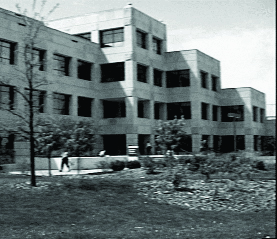
\includegraphics{Images/dc5}

\isucaption{Durham Centre}
\label{mgraph}
\end{figure}

\subsubsection{Parts of the hypothesis}

Here one particular part of the hypothesis that is 
currently being explained is examined and particular
elements of that part are given careful scrutiny.

% Below \subsubsection
% Sectional commands: \paragraph and \subparagraph may also be used

\subsection{Second Hypothesis}

Here one particular hypothesis is explained in depth
and is examined in the light of current literature.

\subsubsection{Parts of the second hypothesis}

Here one particular part of the hypothesis that is 
currently being explained is examined and particular
elements of that part are given careful scrutiny.

\section{Criteria Review}

Here certain criteria are explained thus eventually
leading to a foregone conclusion.


% Chapter 5 from the standard thesis template
%   with a full page figure and a sideways table.
\chapter{SUMMARY AND DISCUSSION}

This is the opening paragraph to my thesis which
explains in general terms the concepts and hypothesis
which will be used in my thesis.

With more general information given here than really
necessary.

\section{Introduction}

Here initial concepts and conditions are explained and
several hypothesis are mentioned in brief.

Or graphically as seen in Figure~\ref{mgraph2}
it is certain that my hypothesis is true.

\begin{figure}[p!] \centering

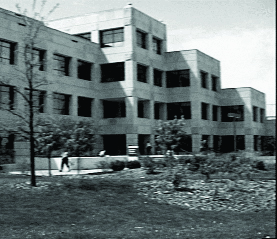
\includegraphics{Images/dc5}

\isucaption{Durham Centre---  Another View}
\label{mgraph2}
\end{figure}

\subsection{Hypothesis}

Here one particular hypothesis is explained in depth
and is examined in the light of current literature.

As can be seen in Table~\ref{nothingelse} it is
truly obvious what I am saying is true.

\begin{sidewaystable} \centering
\isucaption{This table shows almost nothing but is a
sideways table and takes up a whole page by itself}
\label{nothingelse}
% Use: \begin{tabular{|lcc|} to put table in a box
\begin{tabular}{lcc} \hline
\textbf{Element} & \textbf{Control} & \textbf{Experimental} \\ \hline
Moon Rings & 1.23 & 3.38 \\
Moon Tides & 2.26 & 3.12 \\
Moon Walk & 3.33 & 9.29 \\ \hline
\end{tabular}
\end{sidewaystable}

\subsubsection{Parts of the hypothesis}

Here one particular part of the hypothesis that is 
currently being explained is examined and particular
elements of that part are given careful scrutiny.

% Below \subsubsection
% Sectional commands: \paragraph and \subparagraph may also be used

\subsection{Second Hypothesis}

Here one particular hypothesis is explained in depth
and is examined in the light of current literature.

\subsubsection{Parts of the second hypothesis}

Here one particular part of the hypothesis that is 
currently being explained is examined and particular
elements of that part are given careful scrutiny.

\section{Criteria Review}

Here certain criteria are explained thus eventually
leading to a foregone conclusion.


% Appendix1 file from standard thesis template
\appendixtitle
\appendix
\chapter{ADDITIONAL MATERIAL}

This is now the same as any other chapter except that
all sectioning levels below the chapter level must begin
with the *-form of a sectioning command.

\section*{More stuff}

Supplemental material.


% An example second appendix from the example thesis thesis.tex.
\chapter{Developer Survey}

This is now the same as any other chapter except that
all sectioning levels below the chapter level must begin
with the *-form of a sectioning command.

\section*{Survey Questions}

\section*{Survey Responses}

\section*{Survey Statistics}

More stuff.

\renewcommand{\bibname}{\centerline{BIBLIOGRAPHY}}
\unappendixtitle
\newpage
\phantomsection
\addcontentsline{toc}{chapter}{BIBLIOGRAPHY}
\bibliography{mybib}

%% An example bibliography from the standard thesis template
\renewcommand{\bibname}{\centerline{BIBLIOGRAPHY}}
\unappendixtitle
\interlinepenalty=300
% For no page break use thebibnopage environment
\begin{thebibliography}{99}
\addcontentsline{toc}{chapter}{BIBLIOGRAPHY}

\bibitem[Allen, B.~S.~(1984)]{allen}
Allen, B.~S. (1984). System-assigned learning strategies and CBI.
\emph{Journal of Instructional Computing Research},
\emph{1}(1), 3--18.
\filbreak

\bibitem[Bruner, J.~(1960)]{bruner}
Bruner, J. (1960). \emph{The process of education}.
New York: Random House.
\filbreak

\bibitem[Cox, S.~R.~(1974)]{cox}
Cox, S.~R. (1974). Computer-assisted instruction and student performance
in macroeconomic principles.
\emph{The Journal of Economic Education},
\emph{6}(1), 29--37.
\filbreak

\end{thebibliography}

\end{document}
